\chapter{Experiments and Results}
\label{chap:experiments}
This chapter presents a series of experiments designed to answer the research questions posed in \autoref{chap:intro}, focusing on the evaluation of the \acrfull{s6}; \acrfull{vms}. It is evaluated for temporal event spotting in football videos. The accuracy and runtime are compared against the \acrfull{tdeed} baseline; I investigate the impact of feature dimensionality and perform a Bayesian hyperparameter sweep to optimize performance.


\section{Experiment 1: Comparing accuracy}
\label{sec:experiment1}
The first experiment compares accuracy from \acrfull{tdeed} and \acrfull{vms}. The goal is to determine if the \acrshort{vms} model can achieve similar or better accuracy than the \acrshort{tdeed} model. The models are trained on the SoccerNet-V2 dataset \cite{deliege_soccernet-v2_dataset_2021}. They are evaluated using \acrfull{map} and \acrshort{map}@50 metrics.

\subsection{Setup}
\label{ssec:ex1_setup}
% We trained three models on the SoccerNet-V2 dataset \cite{deliege_soccernet-v2_dataset_2021}:  
% \begin{itemize}
%     \item \acrshort{vms}-80\_20 using an 80\%/20\% train/val split,  
%     \item \acrshort{vms}-70\_30 using a 70\%/30\% split, and  
%     \item \acrshort{tdeed} with four matches for training and one for validation (equivalent to 80\%/20\%).  
% \end{itemize}

All models used default hyperparameters from their original papers. Performance was measured by mean \acrfull{map} and \acrshort{map}@50 under a \(\pm1s\) tolerance window (see \cref{sec:eval_protocol}. The dataset was edited accordingly to \cref{sec:preprocessing}, which means the annotations are not equal. 


\subsection{Results}
\label{ssec:ex1_results}
\begin{table}[ht]
    \centering
    \begin{tabular}{lccc}
        \toprule
        Model & average \acrshort{map} (\%)  & validation \acrshort{map}@50 (\%) & test \acrshort{map}@50 (\%)\\
        \midrule
        \acrshort{tdeed} &  \textemdash & 20.78 & \textbf{47.65}\\
        \acrshort{vms} (Mamba-\acrshort{s6})   &  \textbf{50.60}   & 48.26 & 43.80 \\
        \bottomrule
    \end{tabular}
    \caption{Accuracy comparison on SoccerNet-V2.}
    \label{tab:results_ex1}
\end{table}

The \acrshort{vms} model (Mamba-\acrshort{s6}) had an average \acrshort{map} achieving 50.60\%. The \acrshort{tdeed} model's average \acrshort{map} is not calculated as there is no \acrshort{iou}. \acrshort{tdeed}'s validation \acrshort{map}@50 was 20.78\%. In the validation \acrshort{map}@50 category, the \acrshort{vms} model significantly outperformed \acrshort{tdeed}, scoring 48.26\% compared to \acrshort{tdeed}'s 20.78\%.

The \acrshort{tdeed} model achieved a higher test \acrshort{map}@50 of 47.65\%. \acrshort{vms}'s correspondig metric achieved 43.80\%. There is a significant increase from the validation of \acrshort{tdeed}s to its test performance. The same difference is evident from the validation score of \acrshort{tdeed} to \acrshort{vms}'s validation score. \acrshort{tdeed} performs poorly in validation. These results are further investigated in \cref{sec:experiment_6}.

\subsection{Discussion}
\label{ssec:ex1_discussion}

\acrshort{tdeed} performs $3.85\%$ in the test \acrshort{map} compared to \acrshort{vms}. However, I will show how the postprocessing is suboptimal in \acrshort{vms}. By changing a single postprocessing value to increase the test \acrshort{map} by $1.83\%$. I discuss this and other theories on why \acrshort{vms} performs poorly compared to \acrshort{tdeed}. 

Compared with standard benchmarks on other datasets (see \cref{sec:datasets}), the results demonstrate that SoccerNet is neither a difficult nor an easy benchmark to evaluate. However, the Mamba-based RDFA-S6, as well as the \acrshort{vms}, perform well in all categories. The models perform best where \acrlong{sota} \acrshort{map} is lower, likely due to their superior scaling properties when there is limited data available. 

The large difference in validation \acrshort{map}@50 for \acrshort{tdeed} could result from a lack of postprocessing. \acrshort{tdeed} uses two different functions for predicting the test \acrshort{map} and the validation \acrshort{map}. The test evaluator applies \acrfull{snms} to remove redundant detections, while the validation does not remove redundant predictions. Additionally, the validation is performed with a stride of \(2\), whereas the test has a stride of \(1\). With \(fps=25\) and a \(tolerance = \pm1s\), this reduction in temporal resolution hinders the predictions from hitting the tolerance window. 

\begin{figure}[h]
    \centering
    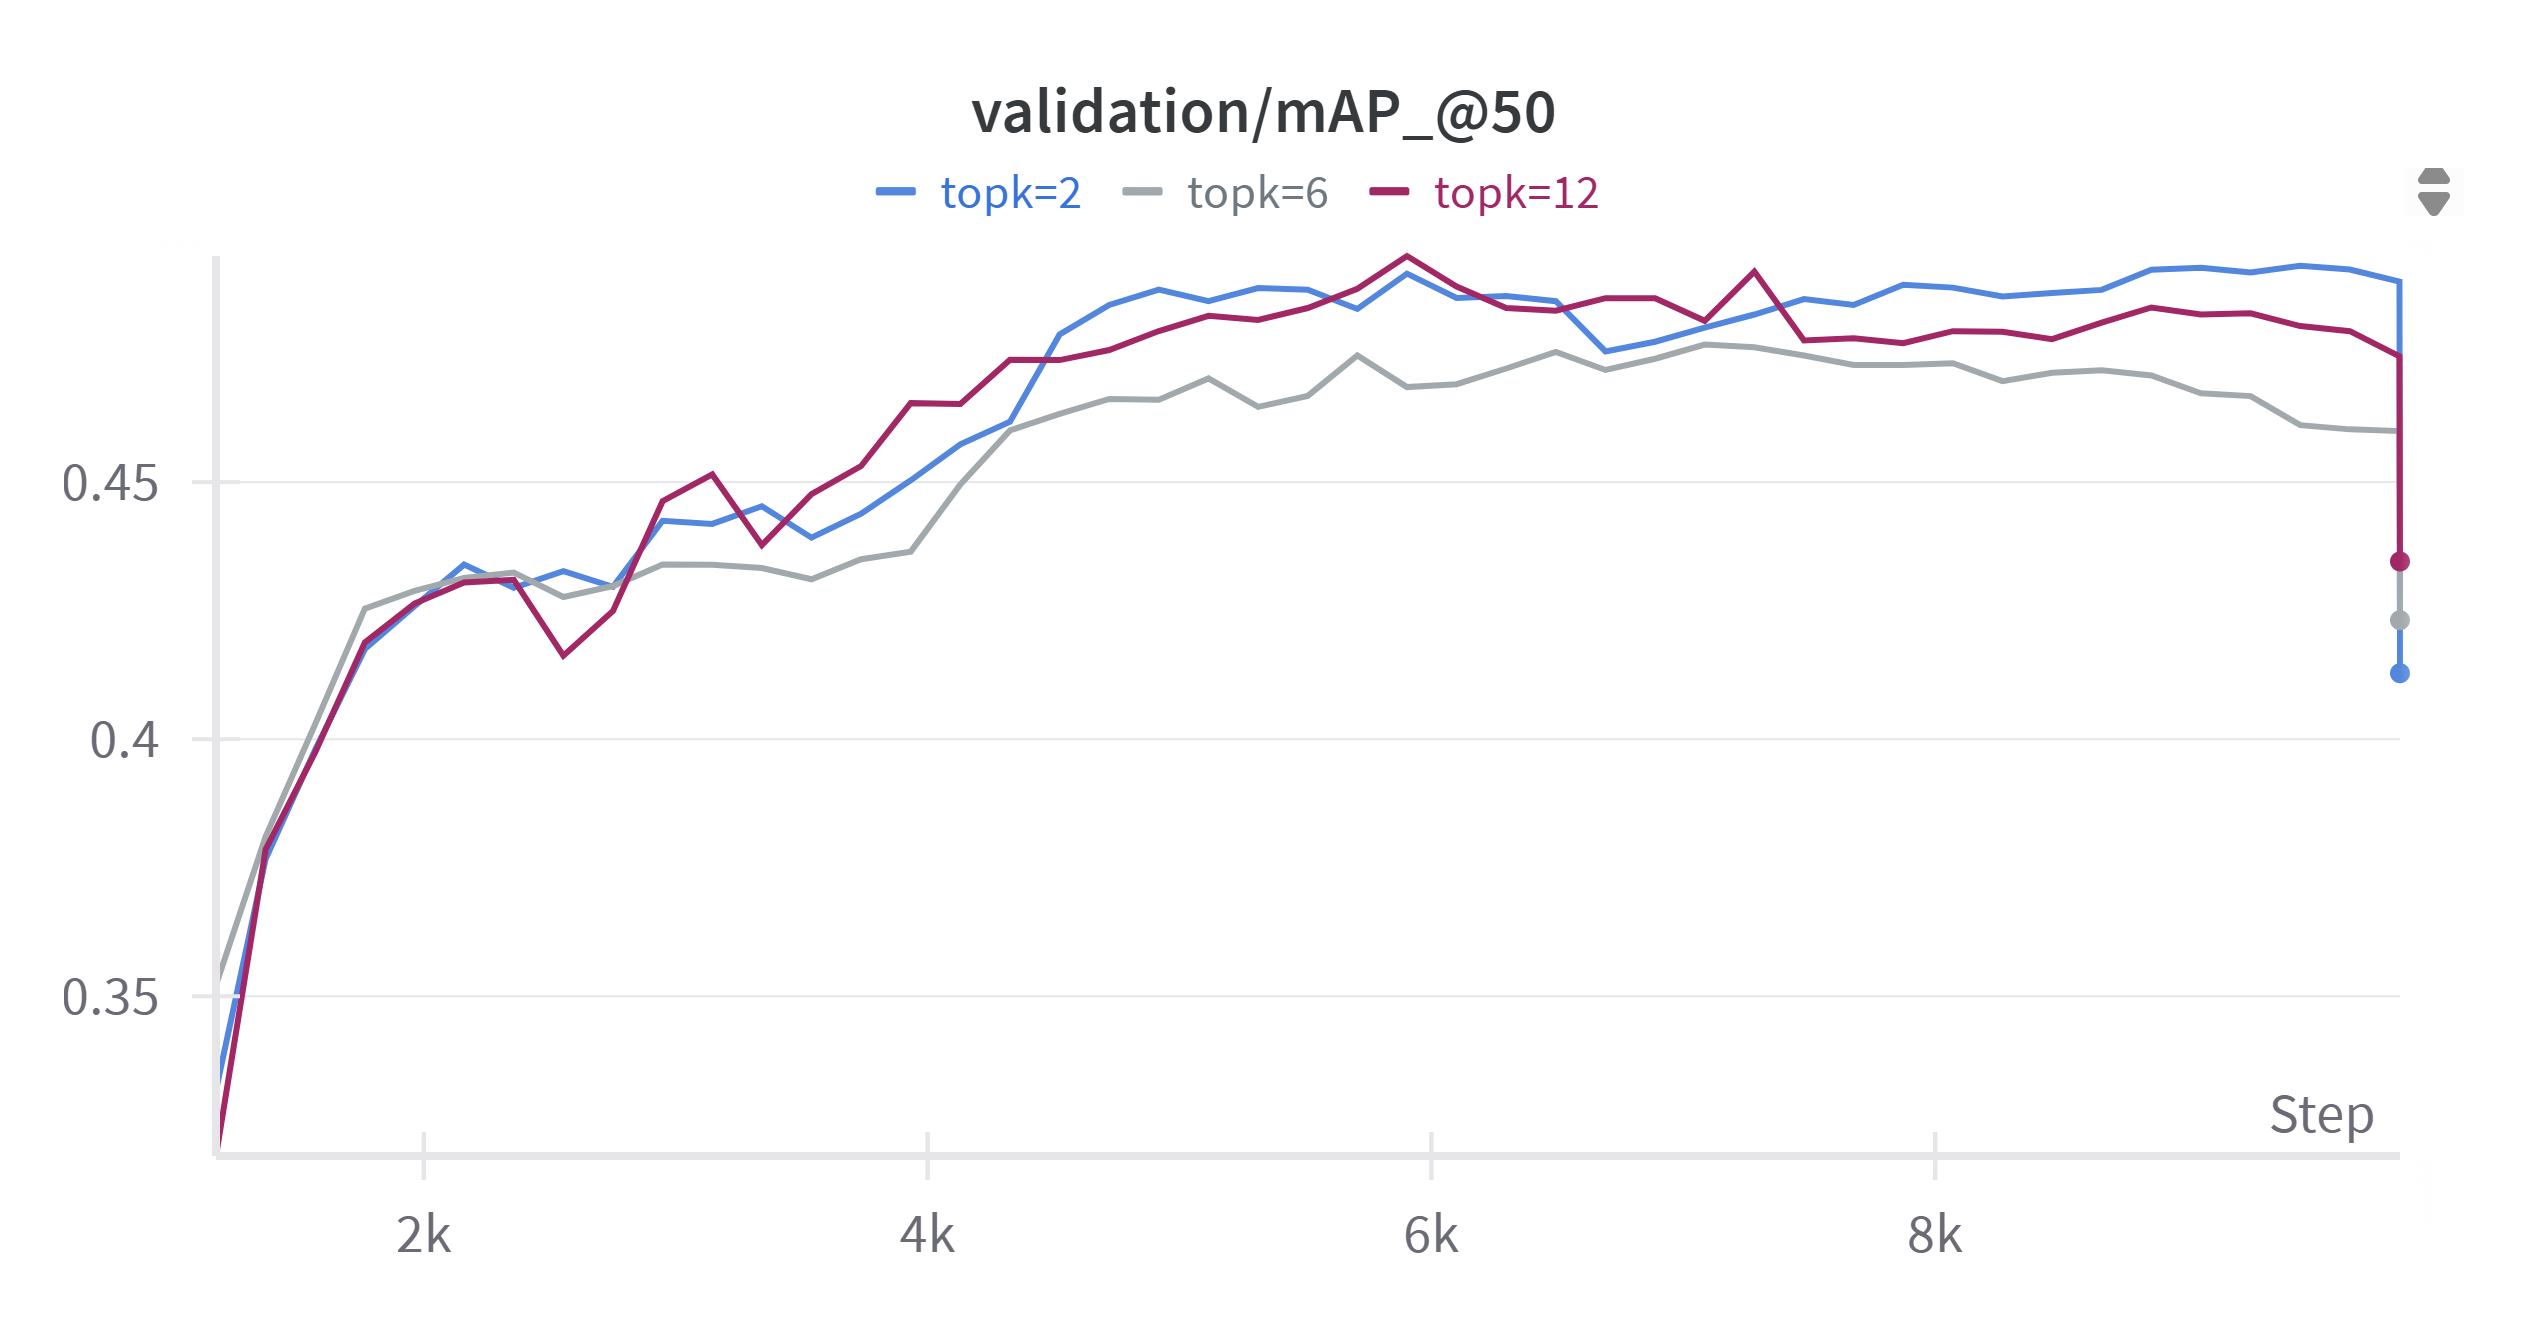
\includegraphics[width=\linewidth]{figures/valid_topk_2.png}
    \caption{Validation plotted per training epoch for the three different values for postprocessing topk. The drop at the end is attributed to the testing results. The test results are described in \cref{fig:topk_test_map}. \(topk=2\) is the default value and is the same run as in \cref{tab:results_ex1}.}
    \label{fig:topk}
\end{figure}

To research if \acrshort{vms} could achieve a similar gain from validation to test by utilizing postprocessing, the postprocessing.py file was modified. The only configurable parameter was the topk. $top (k)$ predicts the $k$ most likely classes to appear within a video.\cref{fig:topk} shows the baseline, which predicts two classes and performs the worst. The increase in value when using six classes is $0.69\%$, and the increase from six to twelve classes is $1.14$. This shows, as expected, that football clips of 1 minute contain a variety of different actions. The baseline value of two likely stems from the nature of YouTube clips, which often involve broader actions. Each video focuses on a single action or two distinct actions. 

\begin{figure}
    \centering
    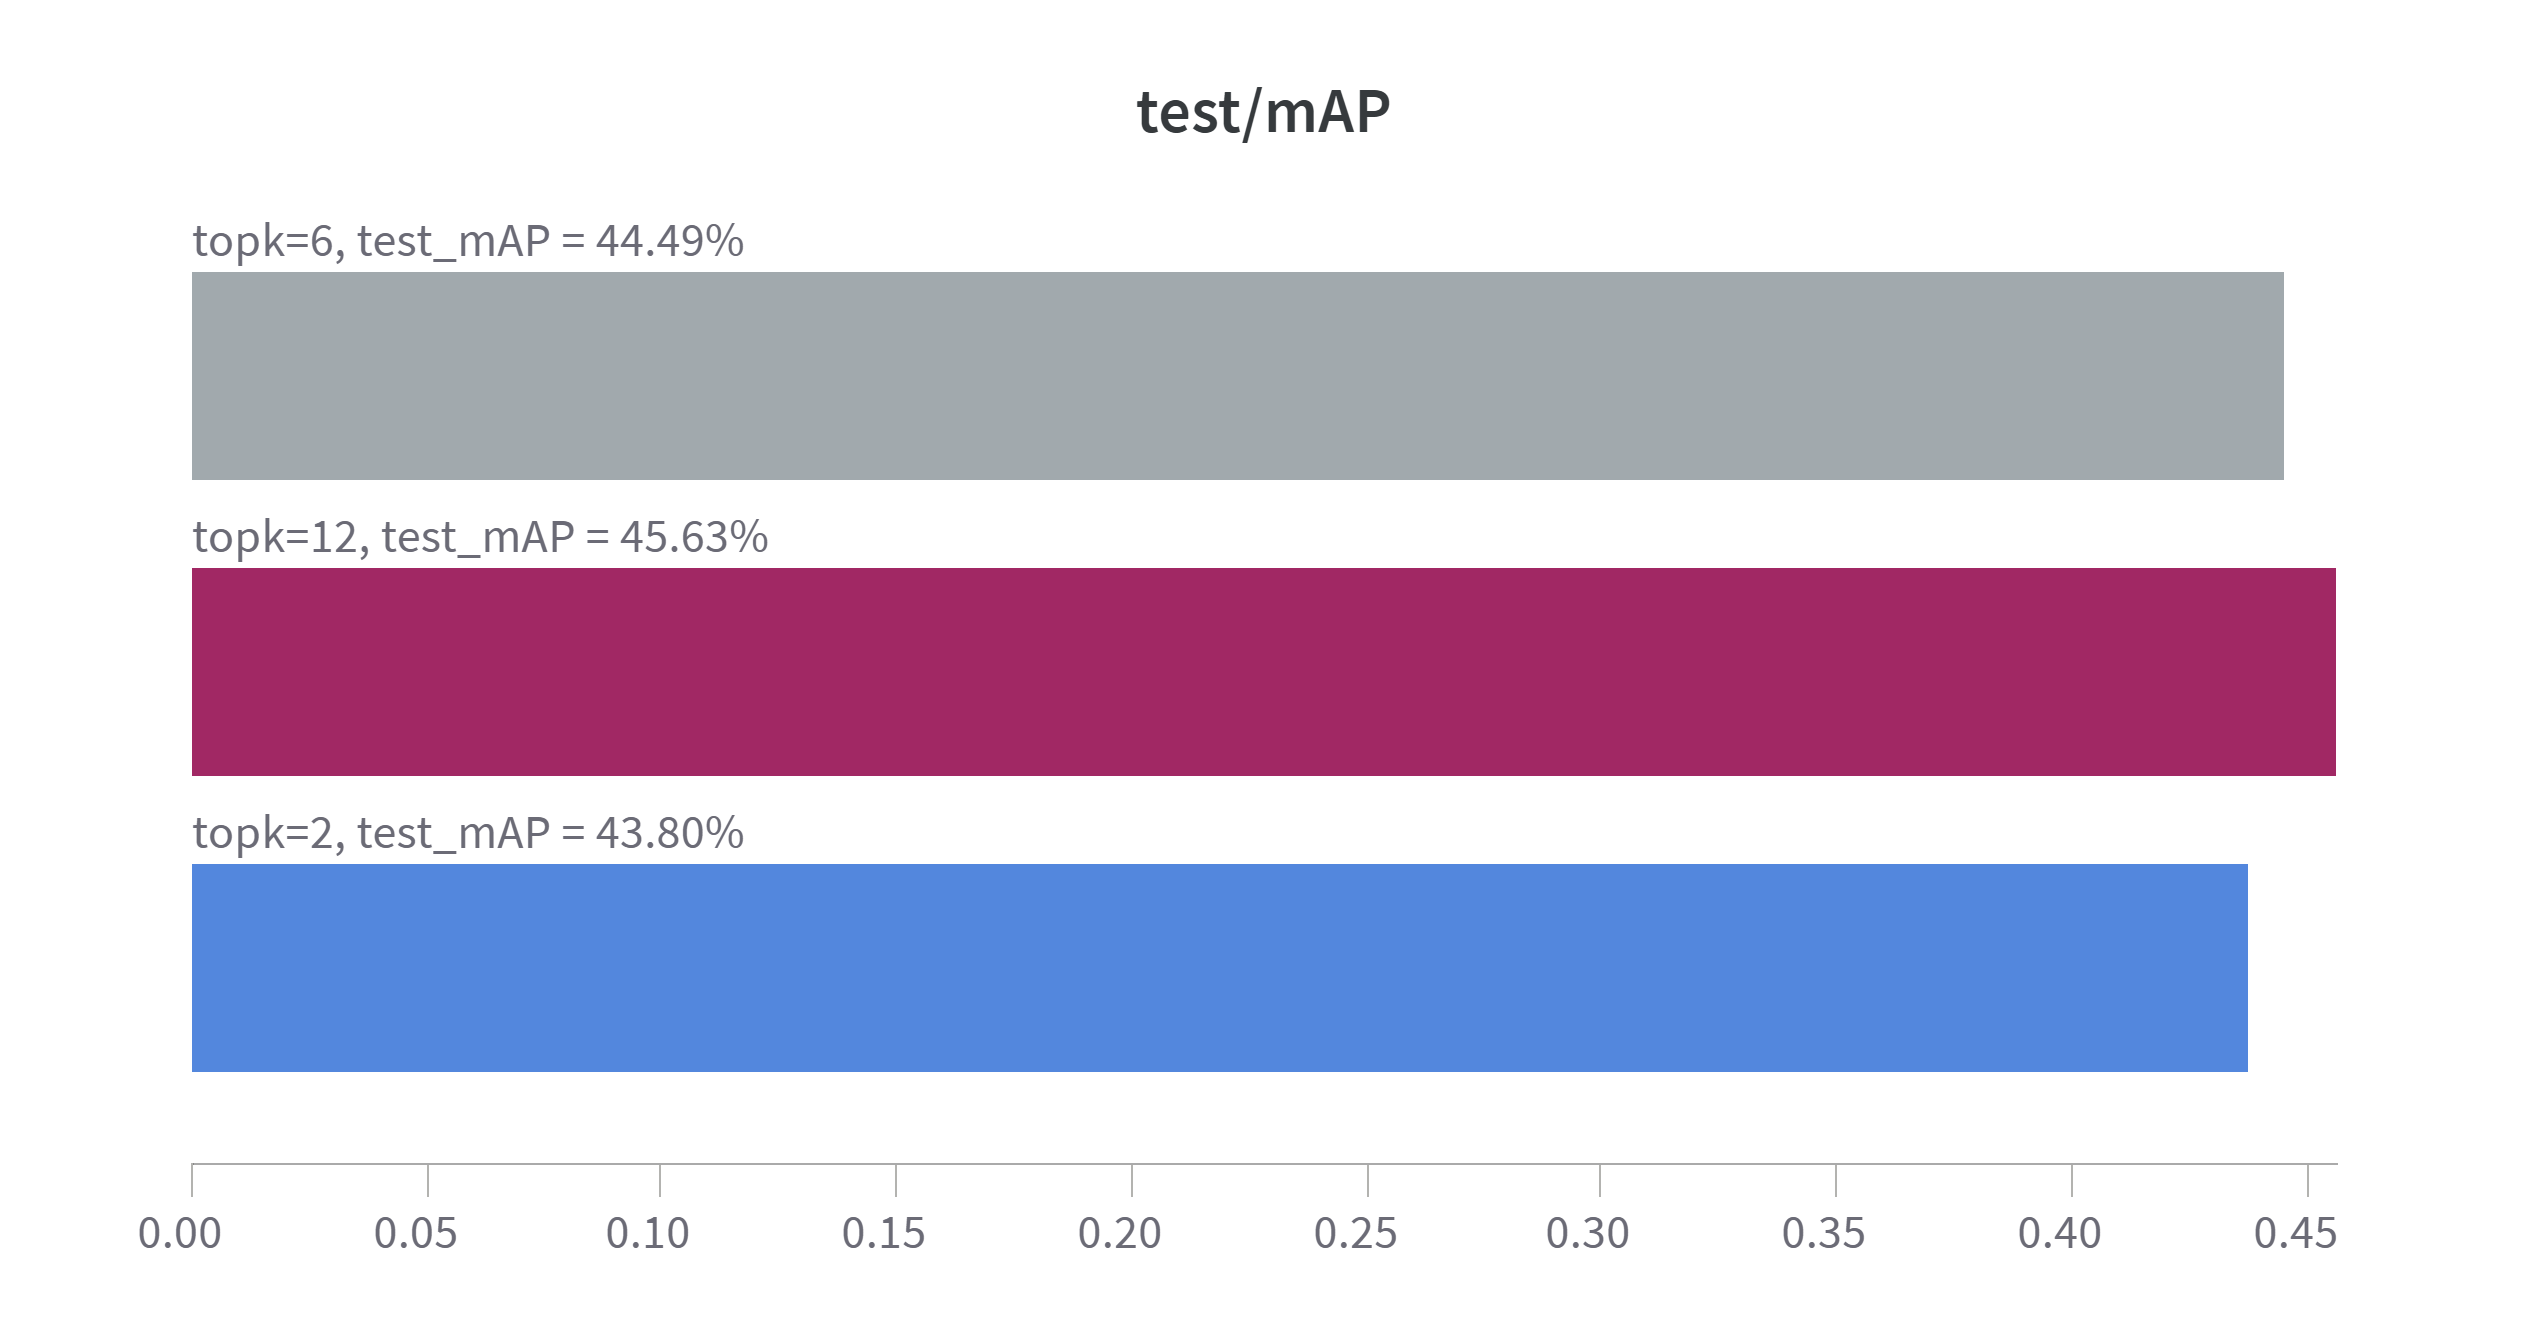
\includegraphics[width=\linewidth]{figures/topk_test_map.png}
    \caption{The results on the test set for each of the different topk configurations. }
    \label{fig:topk_test_map}
\end{figure}

The increase from two, to six, to twelve classes suggests the model is capable of picking up actions that are less prevalent than pass and drive. The dataset is distributed unequally (see \cref{ssec:dataset_soccernet}). An earlier version of this experiment, which was flawed at the start and end of the videos, showed that six classes performed worse, while classes 2 and 12 were equal. The setup does not handle these edge cases sufficiently, but seeing the improvement is interesting. 

There is an interesting observation in \cref{fig:topk}. $topk=2$ consistently outperforms $topk=6$ on the validation set. In later epochs, $topk=2$ outperforms $topk=12$. This is likely due to the distinct nature of games. Some games will have a higher concentration of passes and drives, while others offer a more diverse range of classes.

Using a shorter stride for validation is a technique to increase training speed. In the case of the \acrshort{tdeed} implemented for SoccerNet, the testing phase is weighted more heavily than validation, as it involves submitting to a challenge. A run with \(STRIDE=1\) to discuss this issue in more depth is elaborated in \cref{sec:experiment_6}. 

The temporal discriminability enhancer part of the \acrlong{tdeed} has strategies and components designed to: 
\begin{itemize}
    \item improve the distinction between similar actions
    \item improve token discrimination
    \item give accurate per frame predictions
\end{itemize}

Focusing on temporal distinctions is one key to success in tasks where slight variations in timing or appearance result in different categories. \acrshort{tdeed} is more reactive\todo{not correct word} to small changes in input. In contrast, Mamba's design captures long-range contexts, providing a broader understanding of the video. Mamba is designed to learn more quickly with linear complexity and requires less data.

The validation set size of a single football game can be problematic. Football games can vary significantly due to factors such as team composition, play styles, event frequency, and the referee's threshold for issuing fouls. These are just a few of the variables. There is a risk of bias from the distribution of actions within the validation game. If the validation game is "easy" or "hard," that would severely influence the score. 

While \acrshort{tdeed}'s four matches for training and one for validation is an 80\%/20\% split, validating on a single game can be less representative and more prone to bias than an 80\%/20\% split of clips. The validation set is more robust when the game is split into sections and randomly assigned to either the training or validation set. The result will be more transferable and generalizable. The model with joint training in \cref{fig:500_7_val_compare} has significant variation in its validation performance per epoch. I assume this is because of the inherited differences in validation clips. Some are easy and receive a good validation, while others are hard and perform poorly thereafter. 

The testing set consists of two games from different stadiums. Although the validation issues are also present in testing, testing has twice the data and is more representative of a real-world scenario. Ideally, both problems are mitigated by expanding the dataset. Both extensive augmentation and expanding the dataset are mitigations to this issue, and they are explained further in \cref{sec:future_work}. The test set must also provide the fairest comparison, and therefore, it is not edited. 

\acrshort{vms} runs on any \acrshort{gpu}, but \acrshort{tdeed} needs a lot of memory and only runs on premium \acrshort{gpu}s. If computational resources (especially \acrshort{gpu} memory and type) are a limiting factor, \acrshort{vms} is the more practical choice. \acrshort{vms} has a better GitHub page that explains the installation steps. Although installing the hardware-aware Mamba blocks, which speed up processing times, is challenging, it is a solvable one-time problem.


The \acrshort{tdeed} model was evaluated differently for validation and testing. The validation used a stride of two (halving temporal resolution) and lacked significant postprocessing (such as \acrshort{snms}). The test evaluation used a smaller stride and included such postprocessing. 


Using default hyperparameters from their original papers might not be optimal for the specific SoccerNet-V2 dataset. These defaults might have been tuned for different datasets or tasks, potentially disadvantaging one or both models. This is tackled in \autoref{sec:experiment4}.


Experiment shows that \acrshort{tdeed} achieves a better test \acrshort{map}@50 compared to \acrshort{vms}. The discrepancy is a result of several reasons\improvement{better word}. The validation value of the baseline \acrshort{tdeed} model lacks crucial postprocessing steps. The stride and \acrfull{snms} are put into question. The architectural differences favor the low correctness range of the dataset. The \acrshort{vms} does not spot actions, but temporally labels them, which disfavors the model. 

Experiment shows that \acrshort{tdeed} achieves a better test \acrshort{map}@50 compared to \acrshort{vms}, although \acrshort{vms} demonstrates a significantly higher validation \acrshort{map}@50. This discrepancy can be attributed to several factors. Primarily, \acrshort{tdeed}'s validation procedure differs substantially from its testing phase, lacking crucial postprocessing steps like \acrfull{snms} and employing a larger stride. Both of which negatively impact its validation score. \acrshort{vms}'s performance showed sensitivity to its `topk` postprocessing parameter, but not to the same extent as \acrshort{tdeed}'s postprocessing. Architectural differences also play a role: \acrshort{tdeed} is designed for fine-grained temporal discrimination, whereas \acrshort{vms} focuses on capturing long-range context. Furthermore, the representativeness of \acrshort{tdeed}'s single-game validation set is a concern, potentially leading to biased validation scores. Finally, the use of default hyperparameters for both models on the SoccerNet-V2 dataset might not be optimal. \acrshort{vms} is the better choice when computational resources are limited.

\section{Experiment 2: Compare runtime}
\label{sec:experiment2}

Wall-clock training time for each model on a Tesla A100 \acrshort{gpu} was recorded. Feature extraction and inference time were timed. If no \acrshort{gpu} is specified, the A100 is applied. 

\subsection{Setup}
\label{ssec:ex2_setup}

The same runs used in \autoref{sec:experiment1} are measured. \acrlong{wandb}' metric for duration is measured. In addition, the preprocessing pipelines for each model are isolated and measured independently. A validation run is also done to measure the inference time of each model. A100 \acrshort{gpu}s are used, of size 80 GB or 40 GB, with an indifference to interpret the results. 

\subsection{Results}
\label{ssec:ex2_result}

\begin{table}
    \centering
    \begin{tabular}{lccc}
        \toprule 
        Model & Preprocessing (1 game)  & Training(4+1 games) & Inference (1 game) \\
        \midrule
        \acrshort{tdeed} & 13 & 3267 & 8\\
        \acrshort{vms} (Mamba-\acrshort{s6}) & 342 & 43 & 0.1$(7s)$ \\
        \bottomrule
    \end{tabular}
    \caption{Time comparison. All times are measured in minutes. The inference time for \acrshort{vms} is also provided in seconds. The game between Blackburn Rovers and Nottingham Forest, which lasted 96 minutes, took 7 minutes and 47 seconds, with an average of 0.08 seconds per minute-long clip. Inference time assumes the preprocessing is completed.}
    \label{tab:results_ex2}
\end{table}

\cref{tab:results_ex2} shows the time for each step in each model. The total training time for \acrshort{tdeed} is \(13min+3267min= 3280min\). To infer one game with \acrshort{tdeed} takes \(13min + 8min = 21min \). Concurrently, \acrshort{vms} takes \(342min+43min=385min\) to train on five games. Inference time for one game is approximately the same time as the preprocessing of that game, in this case \(342min\). In both cases, full parallelizability is assumed in preprocessing and inference. 

\begin{table}
    \centering
    \begin{tabular}{|c|c|c|}
        \hline
        Match & Time  & \acrshort{gpu}\\
        \hline
        Blackburn Rovers- Nottingham Forest & 5h 51min & Tesla V100-PCIE-32GB \\
        \hline
        Brentford - Bristol City & 5h 42min & Tesla V100-PCIE-32GB \\
        \hline
        Hull City - Sheffield Wednesday & 5h 42min & Tesla V100-PCIE-32GB \\
        \hline
        Leeds United - West Bromwich & 5h 54min & Tesla V100-PCIE-32GB\\
        \hline
        Middlesbrough - Preston North End & 5h 58min & Tesla V100-PCIE-32GB\\
        \hline
        Reading - Fulham & 5h 51min & Tesla V100-PCIE-32GB\\
        \hline
        Stoke City - Huddersfield Town & 10h49min & Tesla P100-PCIE-16GB\\
        \hline
        Wigan Athletic - Birmingham City & 5h32min & Tesla V100-PCIE-32GB \\
        \hline
        Cardiff City - Queens Park Rangers & 5h 45min & Tesla V100-PCIE-32GB \\
        \hline
        \hline
        \textbf{Average}(excluding Stoke v Huddersfield)= & \textbf{5h 47 min} & \textemdash \\
        \hline
    \end{tabular}
    \caption{The preprocessing times for all games. They are preprocessed using the \acrshort{vmae} pipeline. The average excludes the game between Stoke City and Huddersfield Town because it seems to have been a measuring error, making it take twice as long. }
    \label{tab:average_feature_extraction}
\end{table}

\subsection{Discussion}
\label{ssec:ex2_discussion}

MAMBA is exceptionally quick in running inference on the games, and the bottleneck is the feature processing. Suppose the inference is parallelized over each of the $\approx90$ videos, which is possible. The inference of a game would be complete before you can blink \cite{bartoshuk_blinking_1977}. Quick. The \acrshort{vmae} preprocessing pipeline is the bottleneck. Efforts should be made to decrease this. 


The same is not true for \acrshort{tdeed}. The model is relatively balanced between preprocessing time and inference time. A complete preprocessing and inference of a game takes 21 minutes. Comparing the full pipeline time between the two, the inference time, which is supposed to be one of the advantages of \acrlong{s6}s, is lost due to preprocessing. 

The direct comparison of preprocessing times (13 min for \acrshort{tdeed} vs. 342 min for \acrshort{vms}) is affected by the hardware difference in \acrshort{gpu}s. The actual difference in preprocessing efficiency on identical hardware might be less pronounced than these numbers suggest. \acrshort{vms} preprocessing would still be considerably longer, even if the \acrshort{gpu}s were equal. 


Both runs were run with early stopping mechanisms. Compare \cref{fig:500_7_val_compare} and \cref{fig:plateu_sweep}; it is evident that both models converge before reaching the last epoch. A more aggressive early stopping would favor the \acrshort{tdeed} model, because of the significantly longer epoch time. The difference in training time is still very significant. The training time of \acrshort{tdeed} also decreases the efficiency of a hyperparameter sweep. If each run takes two days, the effort to tune the \acrshort{tdeed} parameters is considerable. 

While A100 \acrshort{gpu}s of both 40GB and 80GB capacities were utilized, the specific workloads were generally not memory-capacity bound, and any minor runtime variations are not expected to alter the primary conclusions regarding relative model and preprocessing speeds. However, this constitutes a minor uncontrolled variable in the experimental setup. 

The assumption of full parallelization simplifies the comparison by looking at the theoretical maximum throughput. Practical implementations might face limitations that increase the observed times. Parallelization on feature extraction was done by queueing jobs on different \acrshort{gpu}s. Achieving perfect or full parallelization in real-world systems is challenging due to:
\begin{itemize}
    \item \textbf{Overhead}: Costs of managing parallel tasks (e.g., data distribution, synchronization).
    \item \textbf{Bottlenecks}: Parts of the pipeline that cannot be parallelized (e.g., serial I/O operations, certain algorithmic steps).
    \item \textbf{Resource Limits}: Finite number of CPU cores, \acrshort{gpu} cores, or memory bandwidth.
\end{itemize}

For research involving frequent retraining or inference on already processed data, \acrshort{vms}'s model speed is a significant advantage. For deploying a model to process new, unseen games quickly from raw video to final output, \acrshort{tdeed}'s faster preprocessing currently gives it an edge in total time, despite its slower model component. The comparison is also impacted by: 

\begin{itemize}
    \item The missing test \acrshort{map}@50 for \acrshort{vms}.
    \item The different GPUs used for measuring \acrshort{vms} preprocessing (V100s) versus \acrshort{tdeed} components (A100s).
    \item The inconsistencies in \acrshort{tdeed}'s validation and test procedures noted in Experiment 1
\end{itemize}

While a P100 \acrshort{gpu} is expected to be slower, the processing time of the Stoke City game was anomalously long. It was excluded from the average sum to provide a more representative preprocessing time for \acrshort{vmae}. The fact that it is $\approx2x$ times the time of the other runs suggests other issues. 

\section{Experiment 3: Feature increase}
\label{sec:experiment3}
To determine the impact of feature vector size, a \acrshort{vms} model with 1408 features and one with 3200 features were trained on the THUMOS-14 dataset.
InternVideo features have a size of 3200 and are the backbone of the \acrshort{sota} models on paperswithcode. The \acrshort{vms} models trained on Soccernet, used in the other experiments, use 1408 features. Both models are trained with a Tesla V100-PCIE-32GB.


\subsection{Setup}
\label{ssec:ex3_setup}

To assess the effect of embedding size, two \acrshort{vms} instances were trained on THUMOS-14\cite{dataset:thumos}: one using 1,408-dimensional VideoMAE features and one using 3,200-dimensional InternVideo embeddings. All other settings, annotations, and hyperparameters remained identical.

The metrics are tracked using \acrlong{wandb} and console logs.
Both models were trained for 49 epochs on a Tesla V100-PCIE-32GB \acrshort{gpu}.

\subsection{Results}
\label{ssec:ex3_results}

\begin{figure}
    \centering
    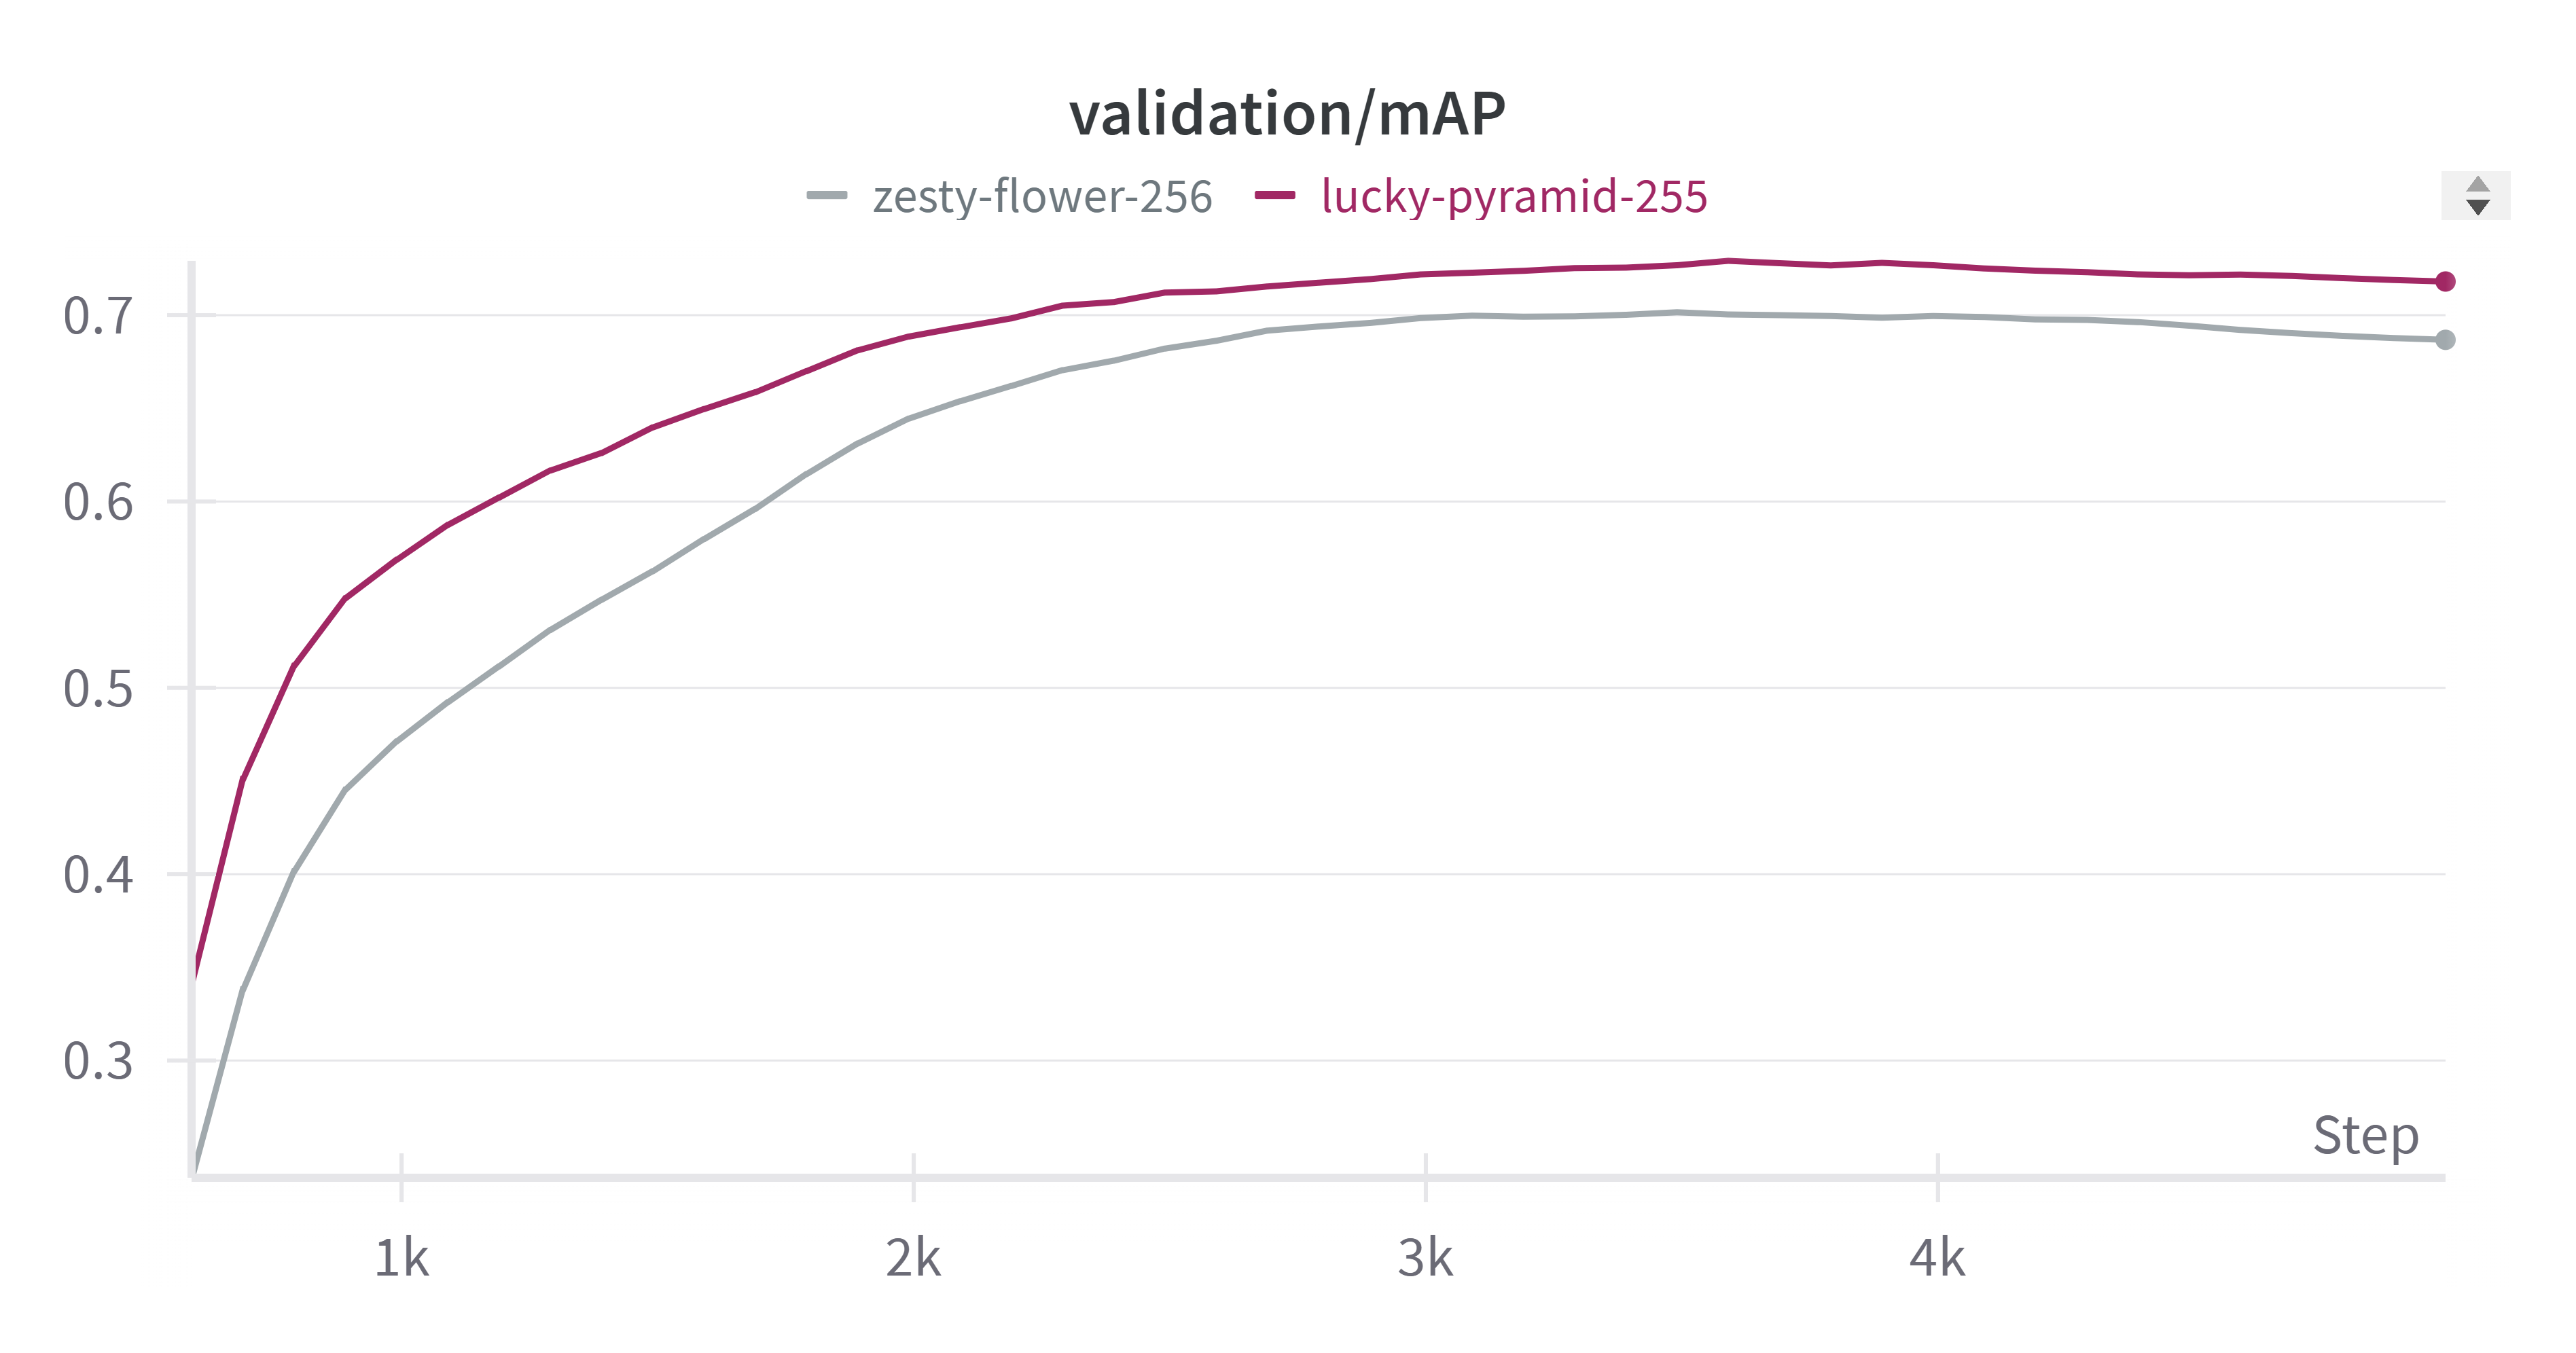
\includegraphics[width=0.75\linewidth]{figures/1408_3200_val.png}
    \caption{Validation per epoch for 3200 features (red) and 1408 features(grey). }
    \label{fig:ex3_val}
\end{figure}
The 1,408-dimensional model achieved a  \acrshort{map} of \(0.686\), while the 3,200-dimensional model reached a \acrshort{map} of \(0.718\) (a 3.2\% absolute gain). Training times were one hour and 15 minutes and 1 hour 23 minutes respectively, an increase of \(\approx11\%\). In \autoref{fig:ex3_val}, you can see how the model with more features outperformed the lower feature model from the first epoch to the last. 


\subsection{Discussion}
\label{ssec:ex3_discussion}

I am confident the $3.2\%$ increase stated in the results is a consistent improvement. As seen in \autoref{fig:ex3_val}, the improvement is consistent over all epochs. The slight drop in the 1408 feature validation score towards the end proves there might be some overfitting in that model, which is not evident in the other model. 

More dimensions inherently increase the probability of linear separability and provide the model with greater capacity to represent complex relationships. 3200 features, as opposed to 1408 features, are more likely to be separable by a simpler model. The increase in features increases the \textit{capacity} for better separation. 

InternVideo features are used in \acrshort{sota} models. This suggests that they are pre-trained in a way that captures very rich and discriminative information relevant to video understanding tasks, such as action recognition. The 3200 dimensions of InternVideo likely encode more fine-grained details, temporal dynamics, or contextual cues than the 1408 dimensions of VideoMAE features. It is not just about having more numbers; these additional numbers represent meaningful variations beneficial for distinguishing actions in THUMOS-14.

In academic research or competitive benchmarking, a $3.2\%$ gain is significant. In the same environments, training times are a secondary concern. As a one-time training, both variants clock in at below 1h30min using a V100 \acrshort{gpu}; this is insignificant in the context of video training. The tradeoff between training time and increased accuracy is favorable. 


\begin{figure}
  \begin{subfigure}{0.42\textwidth}
    \includegraphics[width=\linewidth]{figures/xabi_nigel.png}
        \caption{A foul play, retrieved from Bleacher Report\cite{wyman_2018}.} 
        \label{fig:serious_foul}
  \end{subfigure}%
  \hspace*{\fill}   % maximize separation between the subfigures
  \begin{subfigure}{0.42\textwidth}
    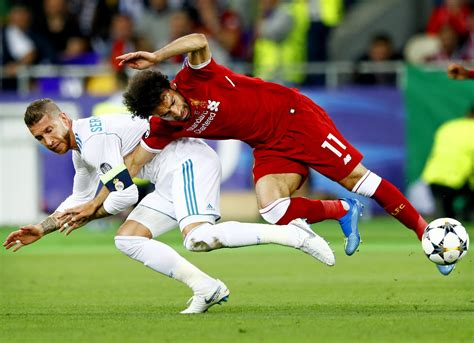
\includegraphics[width=\linewidth]{figures/salah_foul.png}
    \caption{A foul that looks different. Retrieved from The Athletic\cite{corrigan_2021}.} 
    \label{fig:another_foul}
  \end{subfigure}%
  \hspace*{\fill}   
  \caption{Two fouls highlight how unlike 'the same' action can appear. }
  \label{fig:different_fouls}
\end{figure}

Based on the findings from THUMOS-14, where higher dimensionality (3200 features) yielded a 3.2\% absolute \acrshort{map} gain over 1408 features, my hypothesis for football videos is that higher dimensionality would likely be beneficial and potentially even more critical. Football events have significant nuance, as shown in \cref{fig:different_fouls}. At the same time, actions can be homogeneous. \acrshort{cv} does not understand depth in the same way as humans. One of the SoocerNet challenges this year is Monocular Depth Estimation. Understanding whether the ball is in the air(high pass) or on the ground (pass) is difficult. A higher dimensionality can find more hyperplanes to separate these actions on. 

I would hypothesize that the additional descriptive power offered by higher-dimensional features would be advantageous for accurately spotting events in football. More features capture the subtle information needed to spot and classify different events. It could potentially lead to a similar or even greater performance improvement than observed in THUMOS-14 on football videos.

The default hyperparameters are fit to 3200-dimensional features. This may improve its accuracy compared to a default setting for 1408-dimensional features. However, as will be discussed in Experiment 3 in \autoref{sec:experiment3}, hyperparameters are deemed to have little impact. The runs trained on 1408 struggle to improve upon the results from the default parameters. The \acrshort{map} gain could be smaller if hyperparameters were tuned for 1408, but there are no signs that it would be a significant difference from my experiments. 

The 3.2\% absolute \acrshort{map} gain with 3200-dimensional features over 1408-dimensional features suggests that opting for higher-dimensional, more expressive features can lead to significant performance improvements in action spotting. The \(\approx11\%\) increase in training time for the observed accuracy gain is a tradeoff to consider. For applications where accuracy is paramount and the additional training time is acceptable (especially given it was only 8 minutes longer in this specific experiment), using richer features is advisable.


\section{Experiment 4: Hyperparameter optimization}
\label{sec:experiment4}

The fourth experiment is a hyperparameter optimization experiment.
The goal is to find the best hyperparameters for the \acrshort{vms} model on the SoccerNet dataset.

\subsection{Setup}
\label{ssec:ex4_setup}

\acrlong{wandb} is used to track the hyperparameters and results for the \acrshort{vms} model trained on the SoccerNet-V2 dataset with a 70\(\%\)-30\(\%\)- validation split. All seven videos of the SoccerNet V2 format are considered in this approach, including the training, validation, and testing videos. A Bayesian optimization algorithm is used to find the best importance and correlation of the hyperparameters. The hyperparameters related to the dataset are the only ones modified. Full details about the hyperparameter sweeps can be found in \autoref{app:sweep}.

A total of 210 runs across three sweeps of 70 runs each were completed. The hyperparameter search was an efficient process because of the fast convergence of \acrshort{vms}-models. 


\subsection{Results}
\label{ssec:ex4_results}

\begin{figure}[ht]
    \centering
    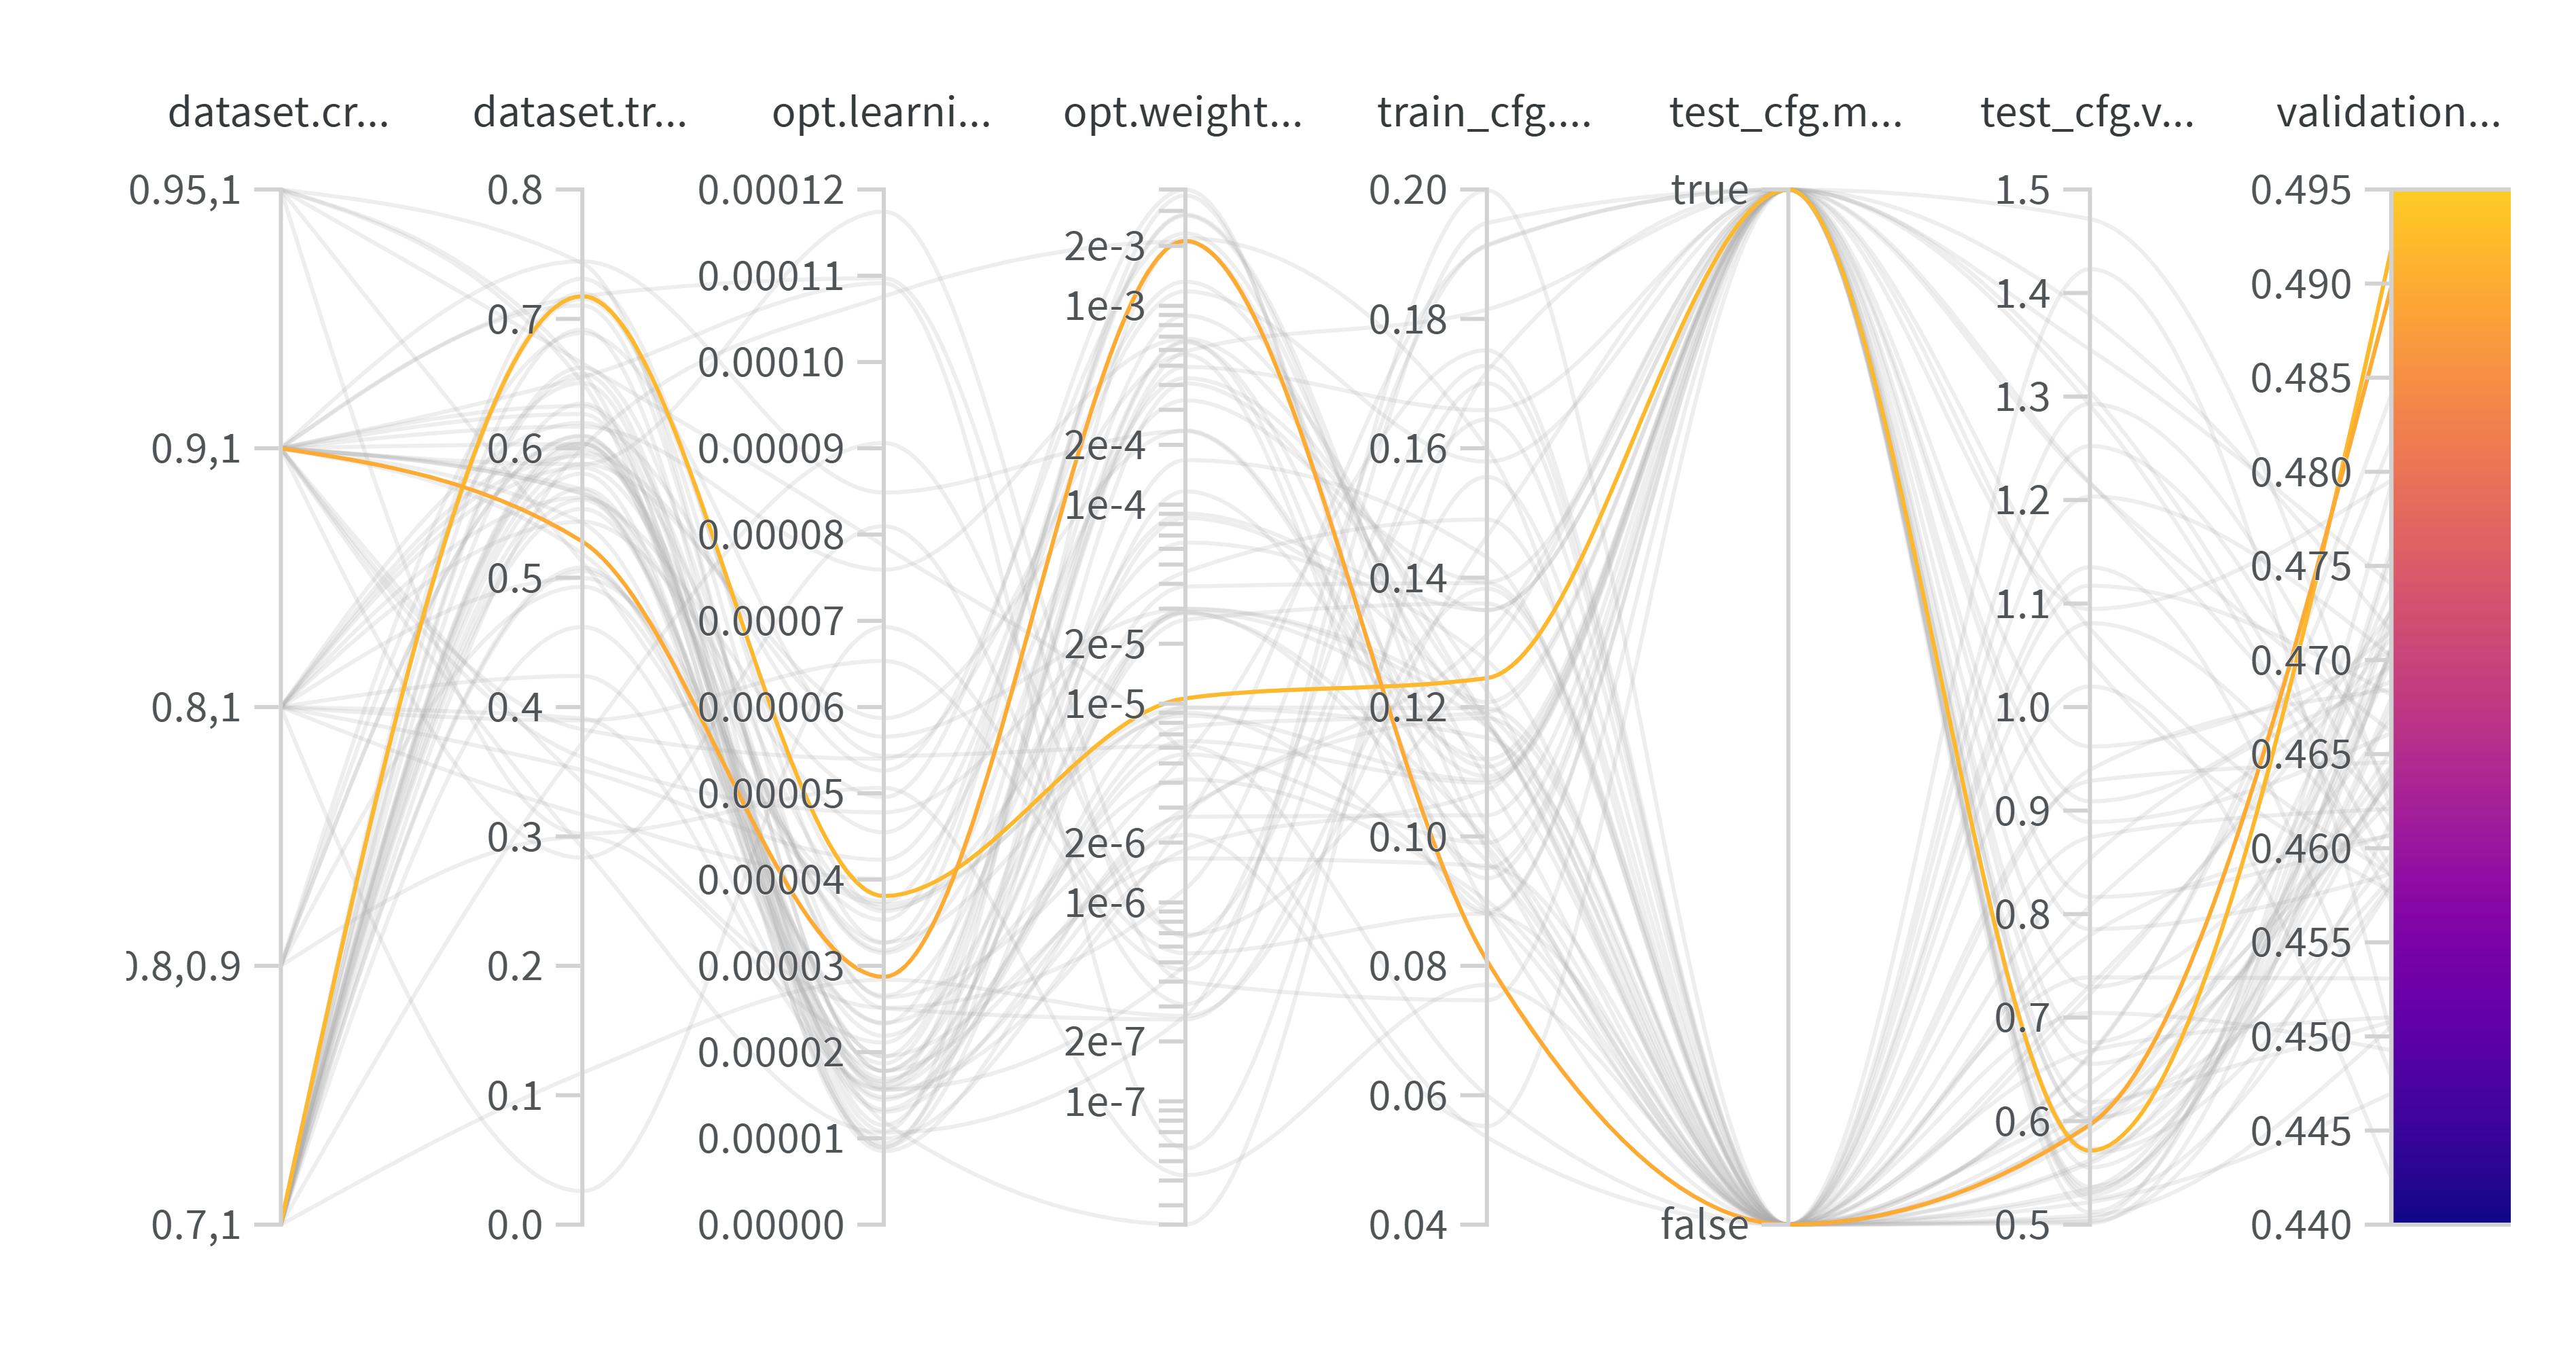
\includegraphics[width=1\linewidth]{figures/sweep_two_best.png}
    \caption{The hyperparameters of the two best results(yellow) compared to all runs (grey) in the third sweep. }
    \label{fig:sweep_best_two}
\end{figure}

The sweeps showed a slight improvement in the model. 

Attempting to translate the sweep into a single, more effective configuration proved unhelpful. However, some configurations performed exceptionally well compared to the rest. These configurations that worked well had quite different parameters, and interpreting which parameters were impactful was difficult. As seen in \autoref{fig:sweep_best_two}, the hyperparameters of the best and second-best runs in the last sweep differed significantly. 

Interpreting the results to create a hyperparameter configuration, as explained in the \autoref{app:sweep_3}, the resulting average \acrshort{map} was \(46.77\%\). 

\subsection{Discussion}
\label{ssec:ex4_discussion}

\begin{figure}
    \centering
    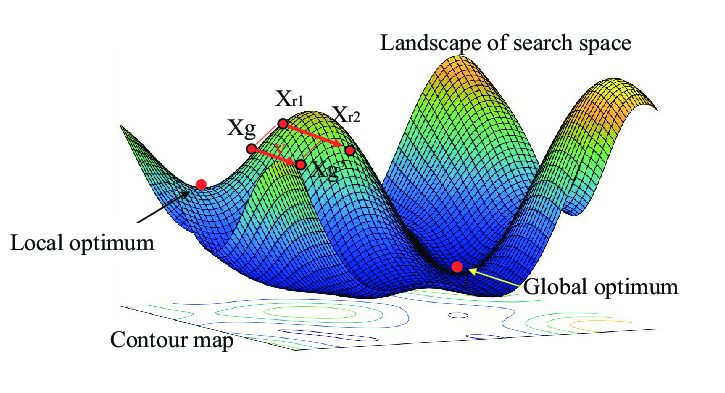
\includegraphics[width=0.75\linewidth]{figures/local_minima.png}
    \caption{A plot of local minima from \cite{fig:multiple_local_minima}. It is not related to any experiments conducted, but its purpose is to serve as a visualization.}
    \label{fig:local_minima}
\end{figure}

It was challenging to translate the sweep into a consistently better configuration despite some exceptional outliers. This likely stems from a few different factors. 

The hyperparameter space might contain multiple local optima. This means there is no single "peak of performance," but rather several combinations of hyperparameters yield good results. Picking an average and combining parameters from distinct optima can result in a configuration. For the sake of visualization, look at \autoref{fig:local_minima} and imagine the summits are optima. Picking an average between them will perform worse than individual peaks. 

Hyperparameters often interact in complex and non-linear ways. The success of an \emph{exceptionally better} configuration might depend on an interplay between multiple parameters. Changing a single parameter in an attempt to generalize or create a "single best" solution might disrupt this delicate balance, leading to suboptimal performance. The fact that the best two runs had "quite different parameters", as seen in \autoref{fig:sweep_best_two}, supports this idea of different, successful combinations rather than a single clear trend.

These two runs imply that multiple good configurations exist. The interaction between the parameters matters more than the individual values. A specific value for one hyperparameter may work well only in conjunction with others. The two good runs in \autoref{fig:sweep_best_two} could represent two good synergies. 

If the hyperparameter landscape had a dominant global optimum, one would expect the best-performing runs to converge towards similar hyperparameter values. The fact that two distinct sets of parameters yield top results suggests that there are at least two separate "peaks" or favorable regions (local optima) in the search space where the model performs exceptionally well. The optimization process has found these different peaks rather than a single point.

This implies some broader challenges for hyperparameter tuning:

\begin{itemize}
    \item Difficulty in Identifying a Single "Best" Configuration: It becomes hard to declare one set of hyperparameters universally optimal. What works best might be one of several good combinations.
    \item Increased Search Complexity: Optimization algorithms can easily get "stuck" in a local optimum, potentially missing a better global optimum or other strong local optima. This necessitates more sophisticated search strategies or more extensive random sampling to explore the space adequately.
    \item Sensitivity to Initial Conditions: The starting point of a hyperparameter search can heavily influence which local optimum is discovered.
    \item Challenges in Interpretation: It is more difficult to draw simple conclusions about the individual impact of each hyperparameter, as their optimal values may be highly dependent on the values of other interacting parameters, leading to different "optimal" combinations.
    \item Reproducibility and Generalization: A specific local optimum found might be particular to the exact dataset split or even the random seed used during the sweep. Generalizing these findings to slightly different conditions can be more challenging.
\end{itemize}

As seen in \autoref{app:sweep_3}, the best runs in the end show that the learning rate of the top-performing runs was relatively low. The Bayesian search preferred exploring lower learning rates, and especially the third sweep showed that low learning rates performed best. In that sweep, the learning rate had the highest importance and absolute correlation. The correlation was negative. 

A lower learning rate enables the model to make finer adjustments in homogeneous data, such as football actions, where events can be visually similar. This can help it learn the subtle distinguishing features without overshooting the optimal weight configurations in the loss landscape, leading to better discrimination between closely related actions.


The hyperparameters that were tuned are:
\begin{itemize}
    \item learning\_rate
    \item weight\_decay
    \item drop\_path 
    \item batch\_size (explored in Sweep 1, then fixed)
    \item voting\_thresh
    \item trunc\_thresh
    \item crop\_ratio (introduced in Sweep 3)
    \item multiclass\_nms (evaluated in Sweep 3)
    \item max\_seq\_len (explored initially, then ignored)
    \item pre\_nms\_topk (explored initially, then ignored)
    \item clip\_grad\_l2norm (explored initially, then ignored)
\end{itemize}

\textbf{Learning rate} appeared to be the most significant value. While its correlation varied, Sweep 3 indicated that the best performance was concentrated in a particularly low range (around 0.00003-0.00004). 

\textbf{Crop ratio} showed apparent performance differences between its settings. As the data augmentation parameter, it was expected to have a higher impact than it did. 

\textbf{droppath} was the most important with the least correlation in the first sweep. It was tuned in Sweep 2 and selected as a fixed value for Sweep 3. 

Sweep 1 deemed \textbf{batchsize} to be unimportant. Ideal values were found for voting\_thresh and trunc\_thresh in Sweep 3. 

The interpreted sweep configuration achieved an average \acrshort{map} of $46.77\%$. Default parameters on the same dataset yielded an average \acrshort{map} of $48.73\%$. This is a decrease in performance of almost $2\%$. When comparing the same data split (70\%/30\% using all seven videos), the default hyperparameters outperformed the configuration derived from interpreting the sweep results. This suggests that creating a single "interpreted" set of hyperparameters was unsuccessful in finding a configuration superior to the defaults for this specific dataset setup.

The best run in the sweep got a $49.18\%$ average \acrshort{map}. That is $2.41\%$ higher than the interpretation and $0.45\%$ higher than the default parameters. It identifies that the sweep identified some configurations that outperformed the default, but an interpreted result did not exist. 

The features from \acrshort{vmae} are implicitly optimized to represent video information based on the original preprocessing pipeline. The ability to improve performance could be limited if the features are "happiest" when processed in a way that mirrors the feature extraction. The dataset's hyperparameters may be tuned to the feature structure, rather than the feature content. The tuning might then explore variations that do not fundamentally alter or improve upon the information already captured by the features. 

Results indicate that while minor gains are possible through extensive tuning, the default \acrshort{vms} hyperparameters seem to be a very effective starting point for the SoccerNet dataset. The hyperparameter space explored, while yielding some improvements, did not reveal overwhelmingly superior configurations.

\begin{figure}
    \centering
    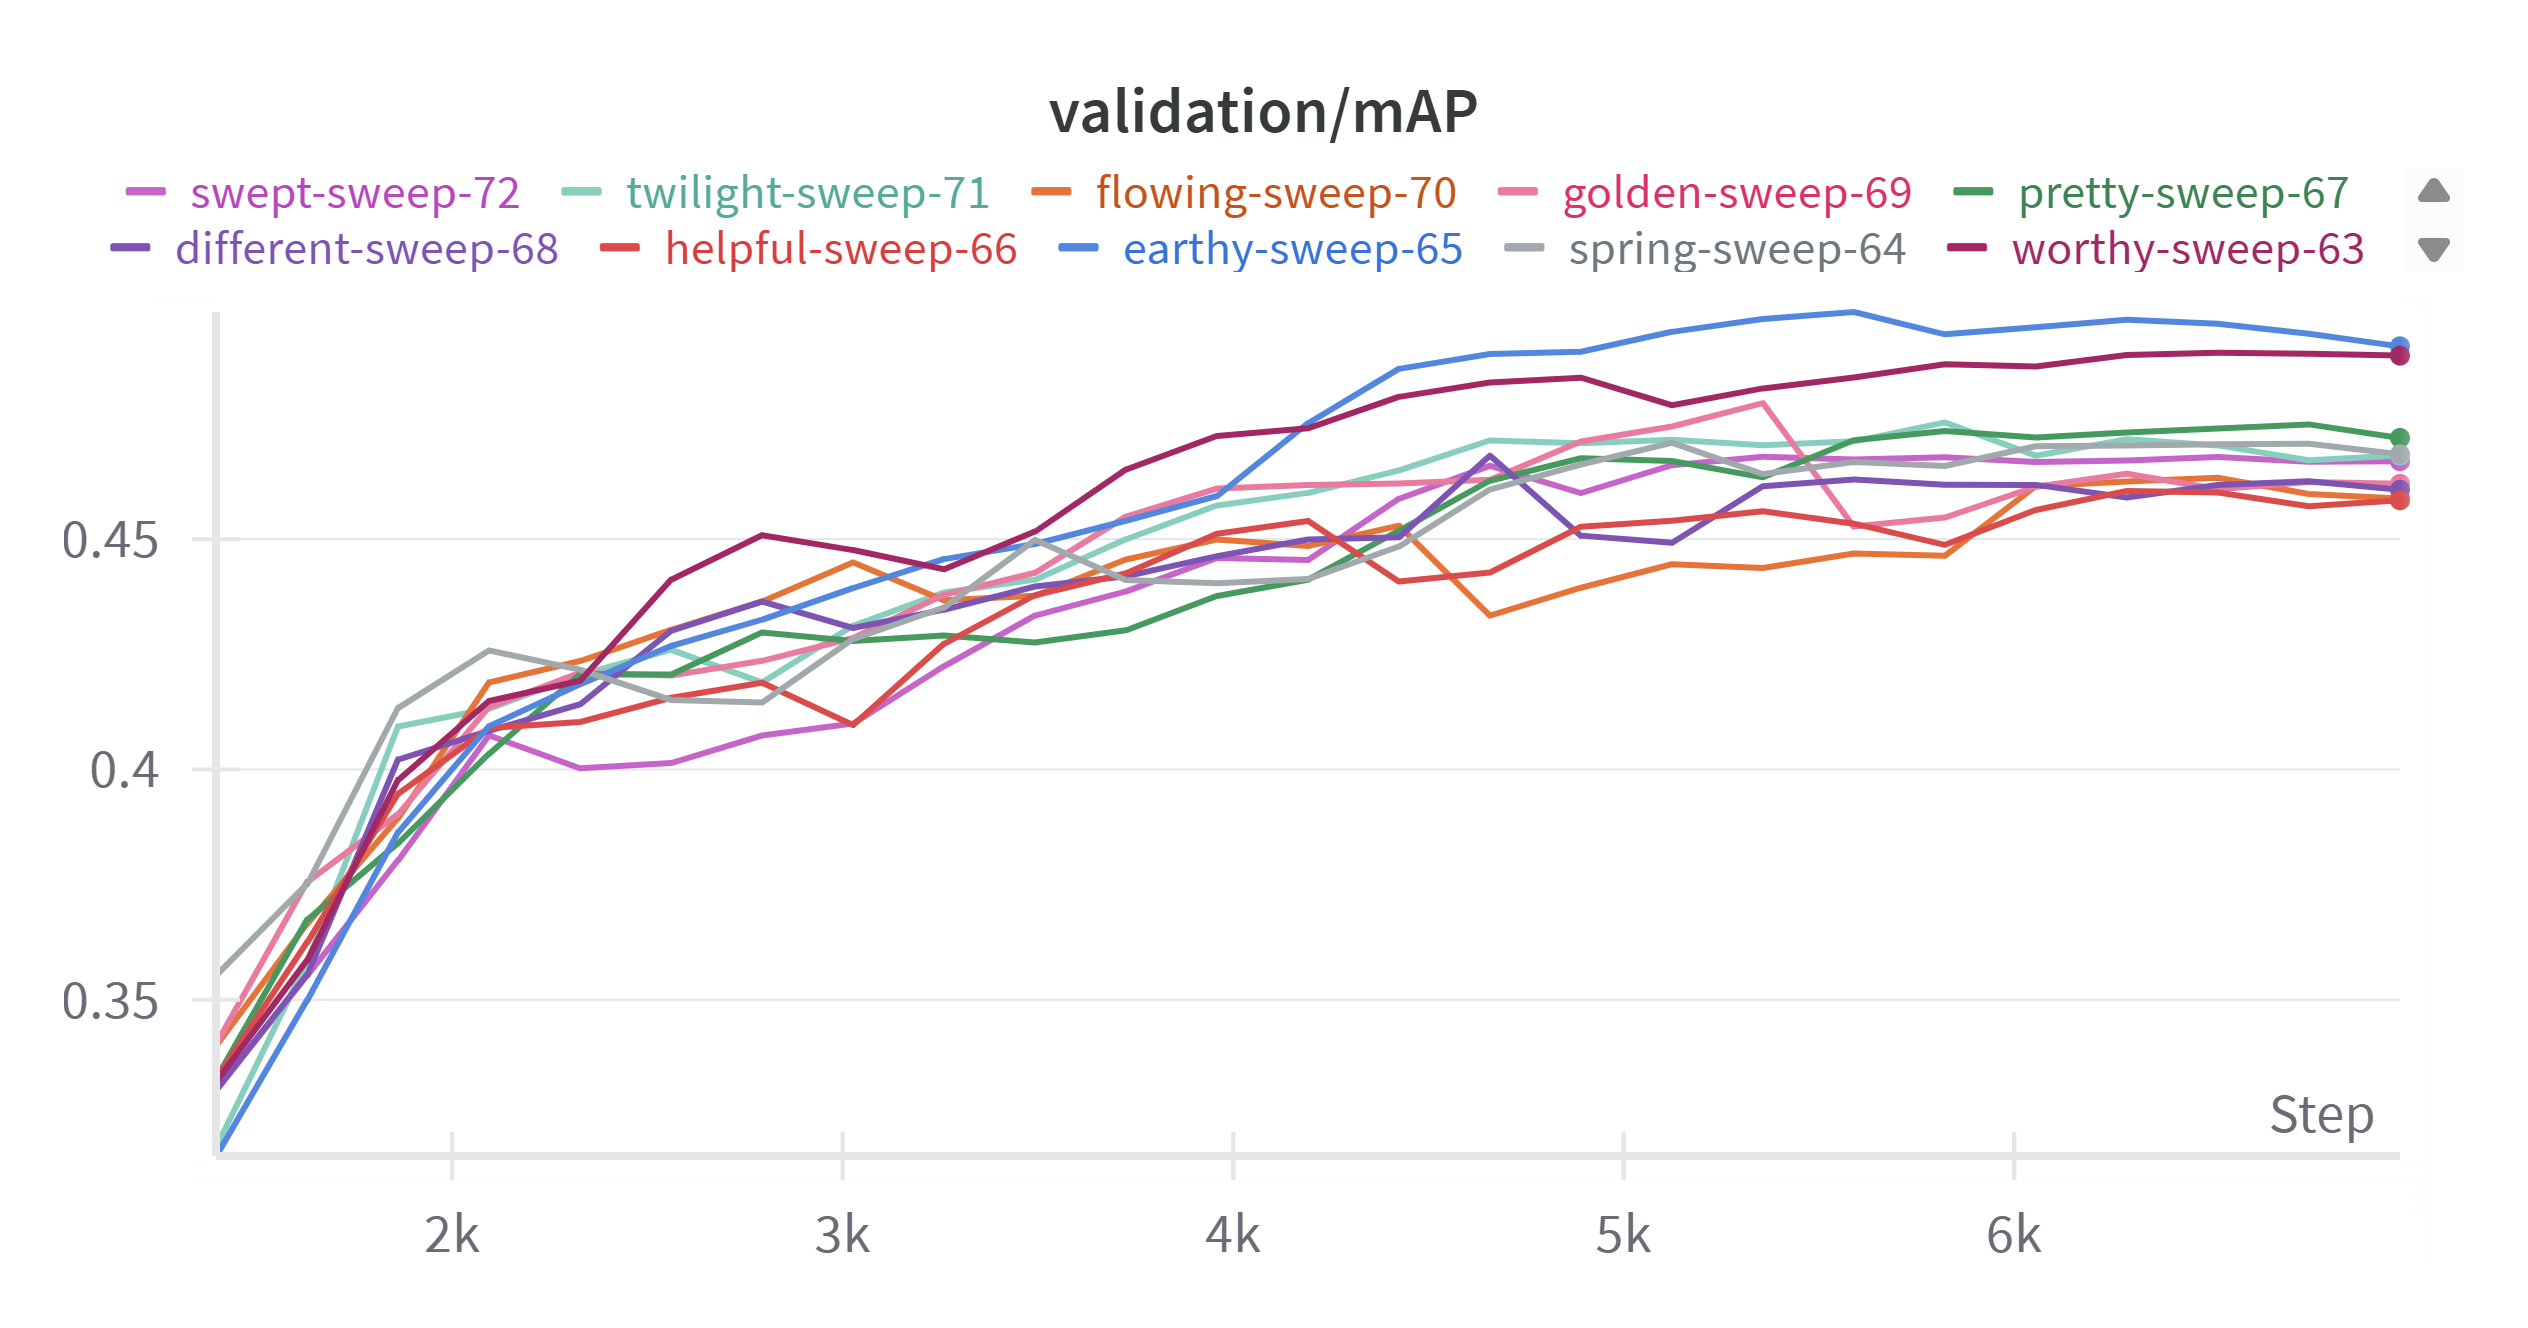
\includegraphics[width=0.75\linewidth]{figures/plateu_sweep.png}
    \caption{Validation plotted against steps for the latest runs in Sweep 3. }
    \label{fig:plateu_sweep}
\end{figure}
\begin{figure}
    \centering
    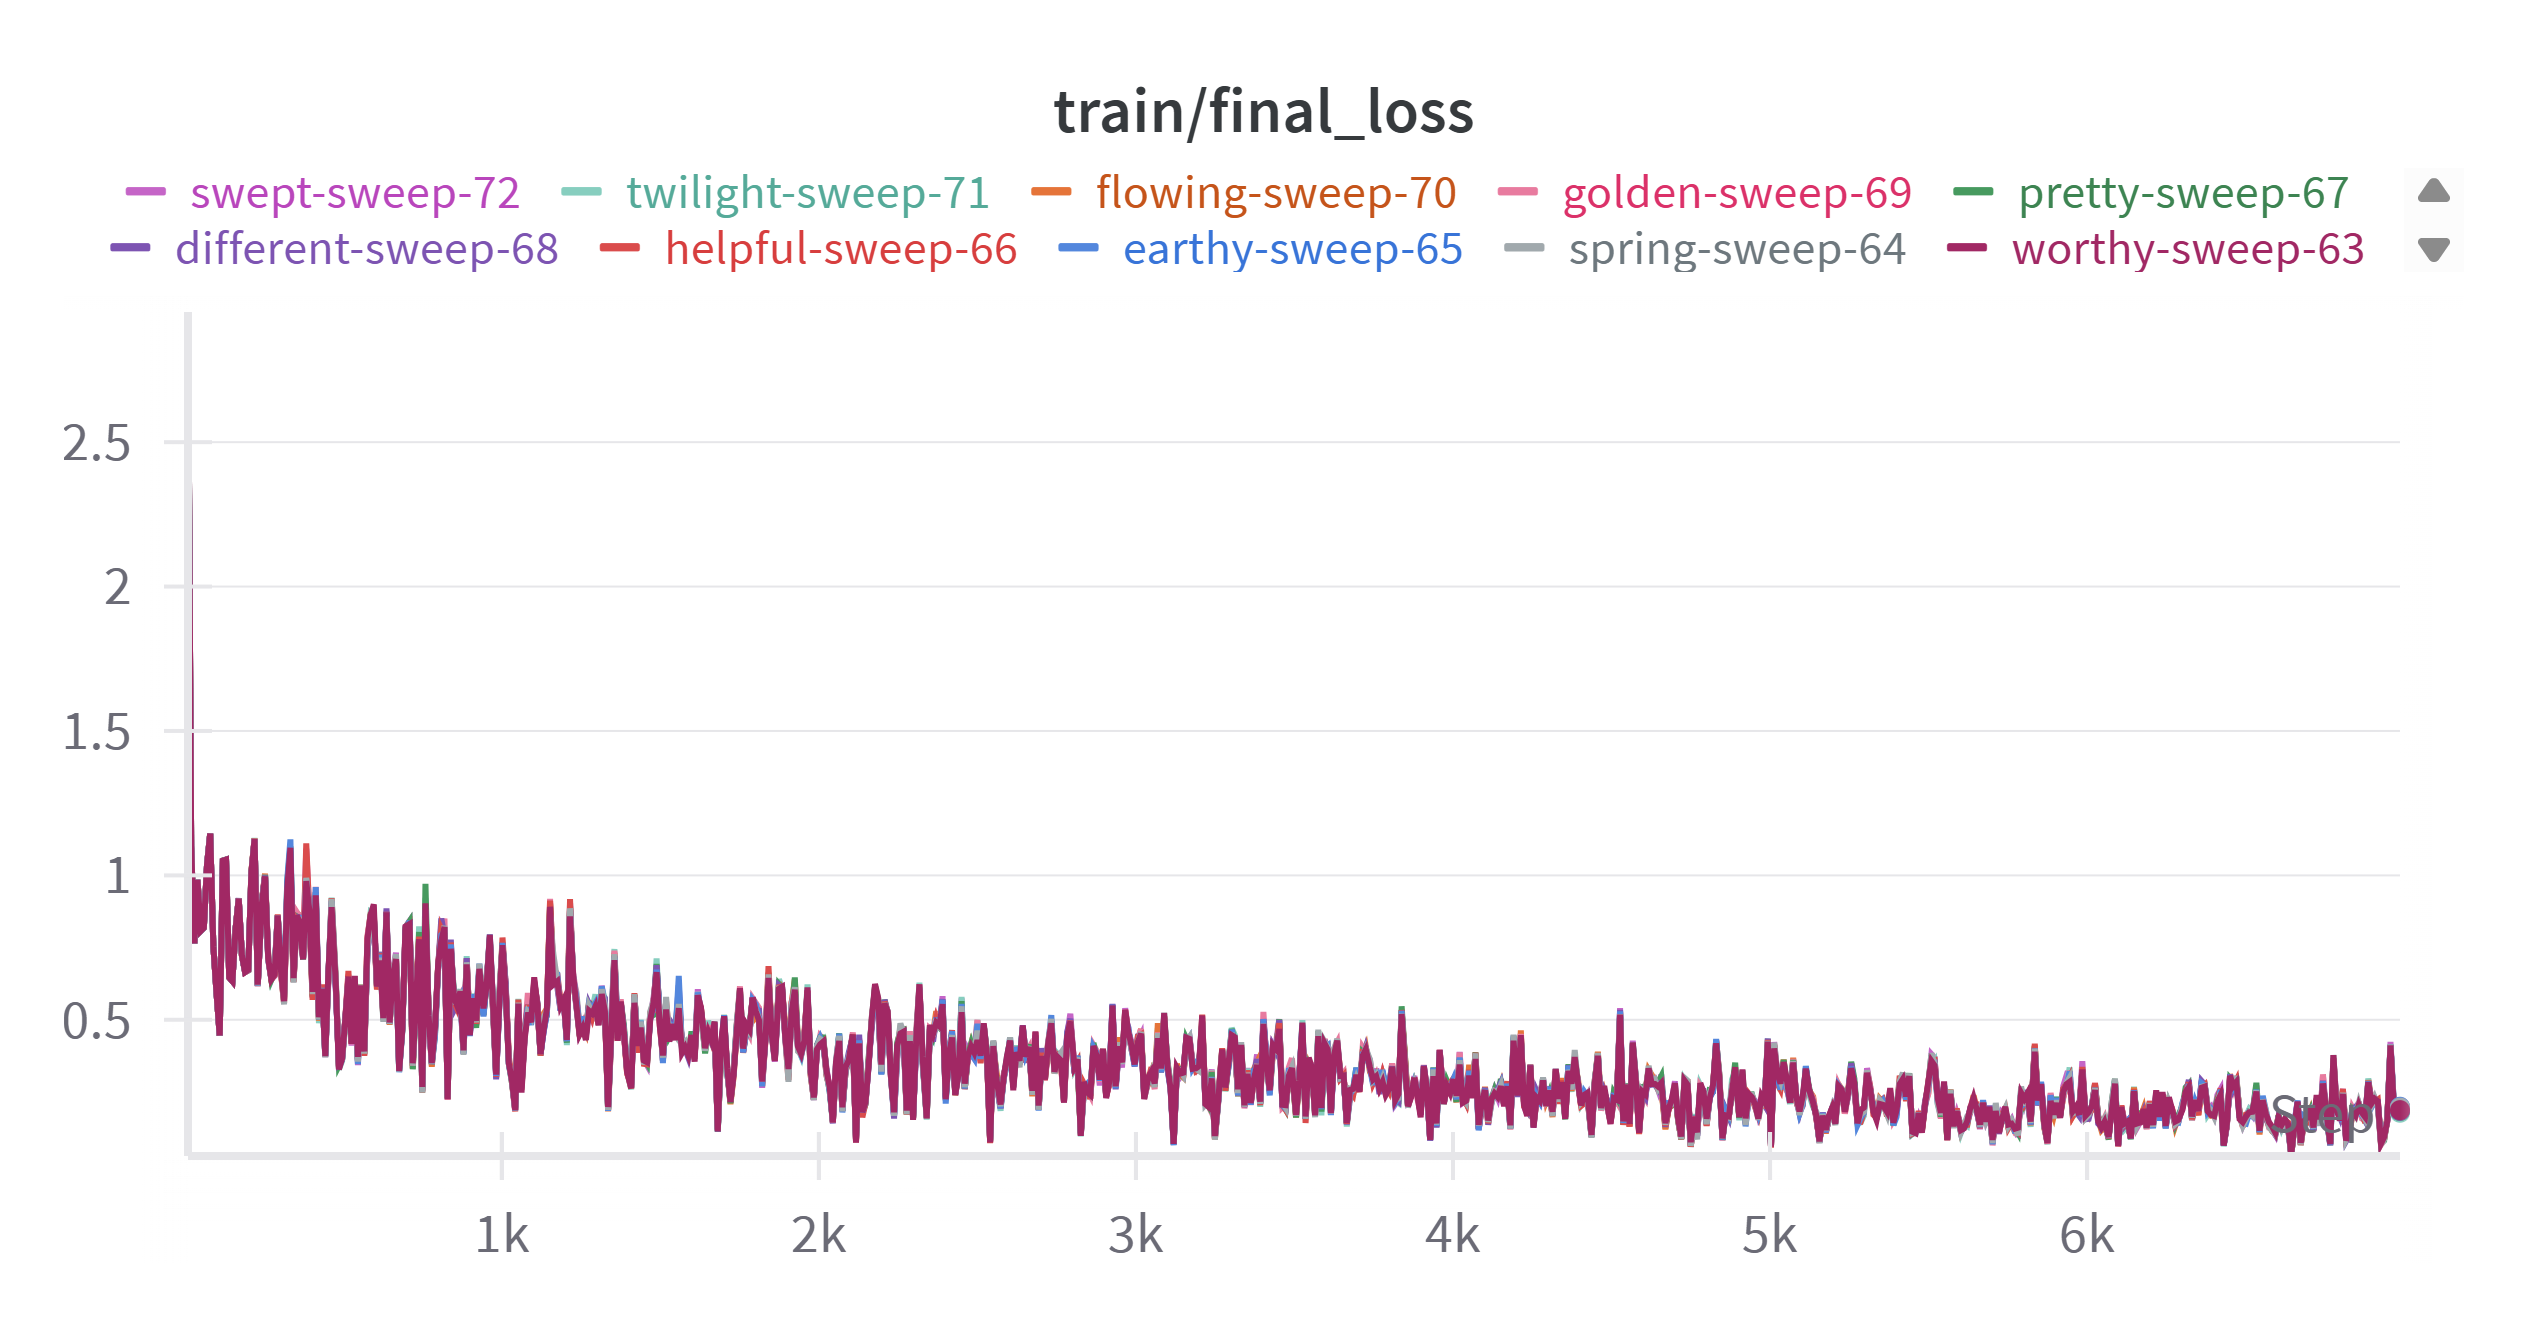
\includegraphics[width=0.75\linewidth]{figures/plateu_loss.png}
    \caption{Training loss plotted against steps for the latest runs in Sweep 3.}
    \label{fig:plateu_loss}
\end{figure}

The general trend of the sweep was for the runs to plateau relatively early, as seen in \autoref{fig:plateu_sweep}. At the same time, the loss was relatively low and stable. This indicates that the model stops generalizing to the validation data and begins to fit to noise in the training data.


Bayesian optimization seeks to identify the optimal hyperparameters in fewer iterations. The algorithm is suited for a landscape with multiple optima because it does not make an inherent assumption of a single optimum. As seen in the Sweeps, some excellent runs were found compared to the average. 

Random search is effective for initial exploration. It has a use case if the initial parameters are considered close to a local optimum, which is not the global optimum. I had no reason to believe this, nor the motivation to explore enough variables compared to the original authors\cite{li_videomamba_2024}.

It might have been beneficial to start with a more extensive exploration before running the Bayesian search. This would require much more than the 210 runs on \acrshort{idun}, which was already under pressure. I find it probable that the default parameters, second \acrshort{sota} on the THUMOS benchmark, are close to the global optima. For sustainability, regarding power usage and the fair use of computational resources, I believe it is correct to discontinue the search. If the results showed a greater increase, the decision would need to be reconsidered.


Experiment 1 mentioned that \textit{Using default hyperparameters from their original papers might not be optimal for the specific SoccerNet-V2 dataset - \cref{ssec:ex1_discussion}.}. Experiment 4 explored this for \acrshort{vms} and found its defaults were already firm. However, \acrshort{tdeed} was not subjected to a similar hyperparameter optimization. Therefore, while there is more confidence that \acrshort{vms}'s default performance is close to its tuned potential on this dataset, the same cannot be said for \acrshort{tdeed}. \acrshort{tdeed} might still have untapped potential if its hyperparameters were similarly optimized for SoccerNet.

To conclude:
\begin{itemize}
    \item \textbf{Default Hyperparameters are Robust}: The default hyperparameters for \acrshort{vms} provide a strong baseline. Extensive tuning might only yield marginal gains, suggesting that the original authors provided well-chosen defaults. This implies that for future comparisons or new experiments, starting with defaults is a reasonable approach, and significant deviations in performance are more likely due to other factors (model architecture, data, etc.) than suboptimal default settings.
    \item \textbf{Hyperparameter Optimization is Complex and Not Always a Silver Bullet}: The search space can have multiple local optima, making finding a single, universally "best" configuration difficult. Creating an "interpreted" best configuration from a sweep might not outperform the defaults or the best individual run found. This cautions against over-reliance on hyperparameter sweeps to unlock performance gains if a model is already well-designed.
    \item \textbf{Learning Rate is a Key Lever, Especially for Homogeneous Data}: For datasets like SoccerNet, where actions can be visually similar, a lower learning rate appears beneficial. This is a takeaway for tuning \acrshort{vms} on such data.
    \item \textbf{Pre-trained Features Influence Tuning}: The characteristics of pre-trained input features can constrain the effectiveness of tuning downstream hyperparameters. The features might already be optimized for a specific processing "timeline," limiting how much dataset-specific tuning can improve things.
    \item \textbf{Resource Constraints and Practicality}: Exhaustive hyperparameter search is computationally expensive. The decision to stop must be balanced against the potential for gains and available resources, especially if initial results suggest diminishing returns.
    \item \textbf{Impact on Comparative Experiments}: The finding that \acrshort{vms} defaults are strong lends more credibility to comparisons made using these defaults (like in Experiment 1). However, it also highlights that the comparison might not reflect its potential if a competing model were not similarly tuned.
    \item \textbf{Focus on Broader Factors}: Given the modest gains from hyperparameter tuning, other factors like feature quality (Experiment 3), model architecture, data augmentation, and postprocessing strategies might offer more significant avenues for performance improvement.
\end{itemize}

\section{Experiment 5: \acrshort{tdeed} with and without joint training}
\label{sec:experiment_5}

The experiment compares two runs using the \acrfull{tdeed} model. The goal is to discover the performance loss by ignoring annotated games for a different action-spotting challenge. 

\subsection{Setup}
\label{ssec:ex5_setup}

\textcite{cioppa_soccernet_2024} provide the implementation of the \acrshort{tdeed} designed to train on all annotated games. The model is adapted to train on the \acrshort{snb} games, not the full dataset. \acrshort{map} per class, validation \acrshort{map}, test loss and compute time are the metrics used. 

The models are run with default hyperparameters and differ only in the dataset size. The difference in the dataset is that the broader classes are present in the grander datasets. There are 12 classes from team events, such as corners and goal kicks. The newer dataset includes annotations indicating whether the left or right team is acting, whereas the older dataset does not. The default hyperparameters are designed for the old challenge. 


\subsection{Results}
\label{ssec:ex5_results}

\begin{figure}
    \centering
    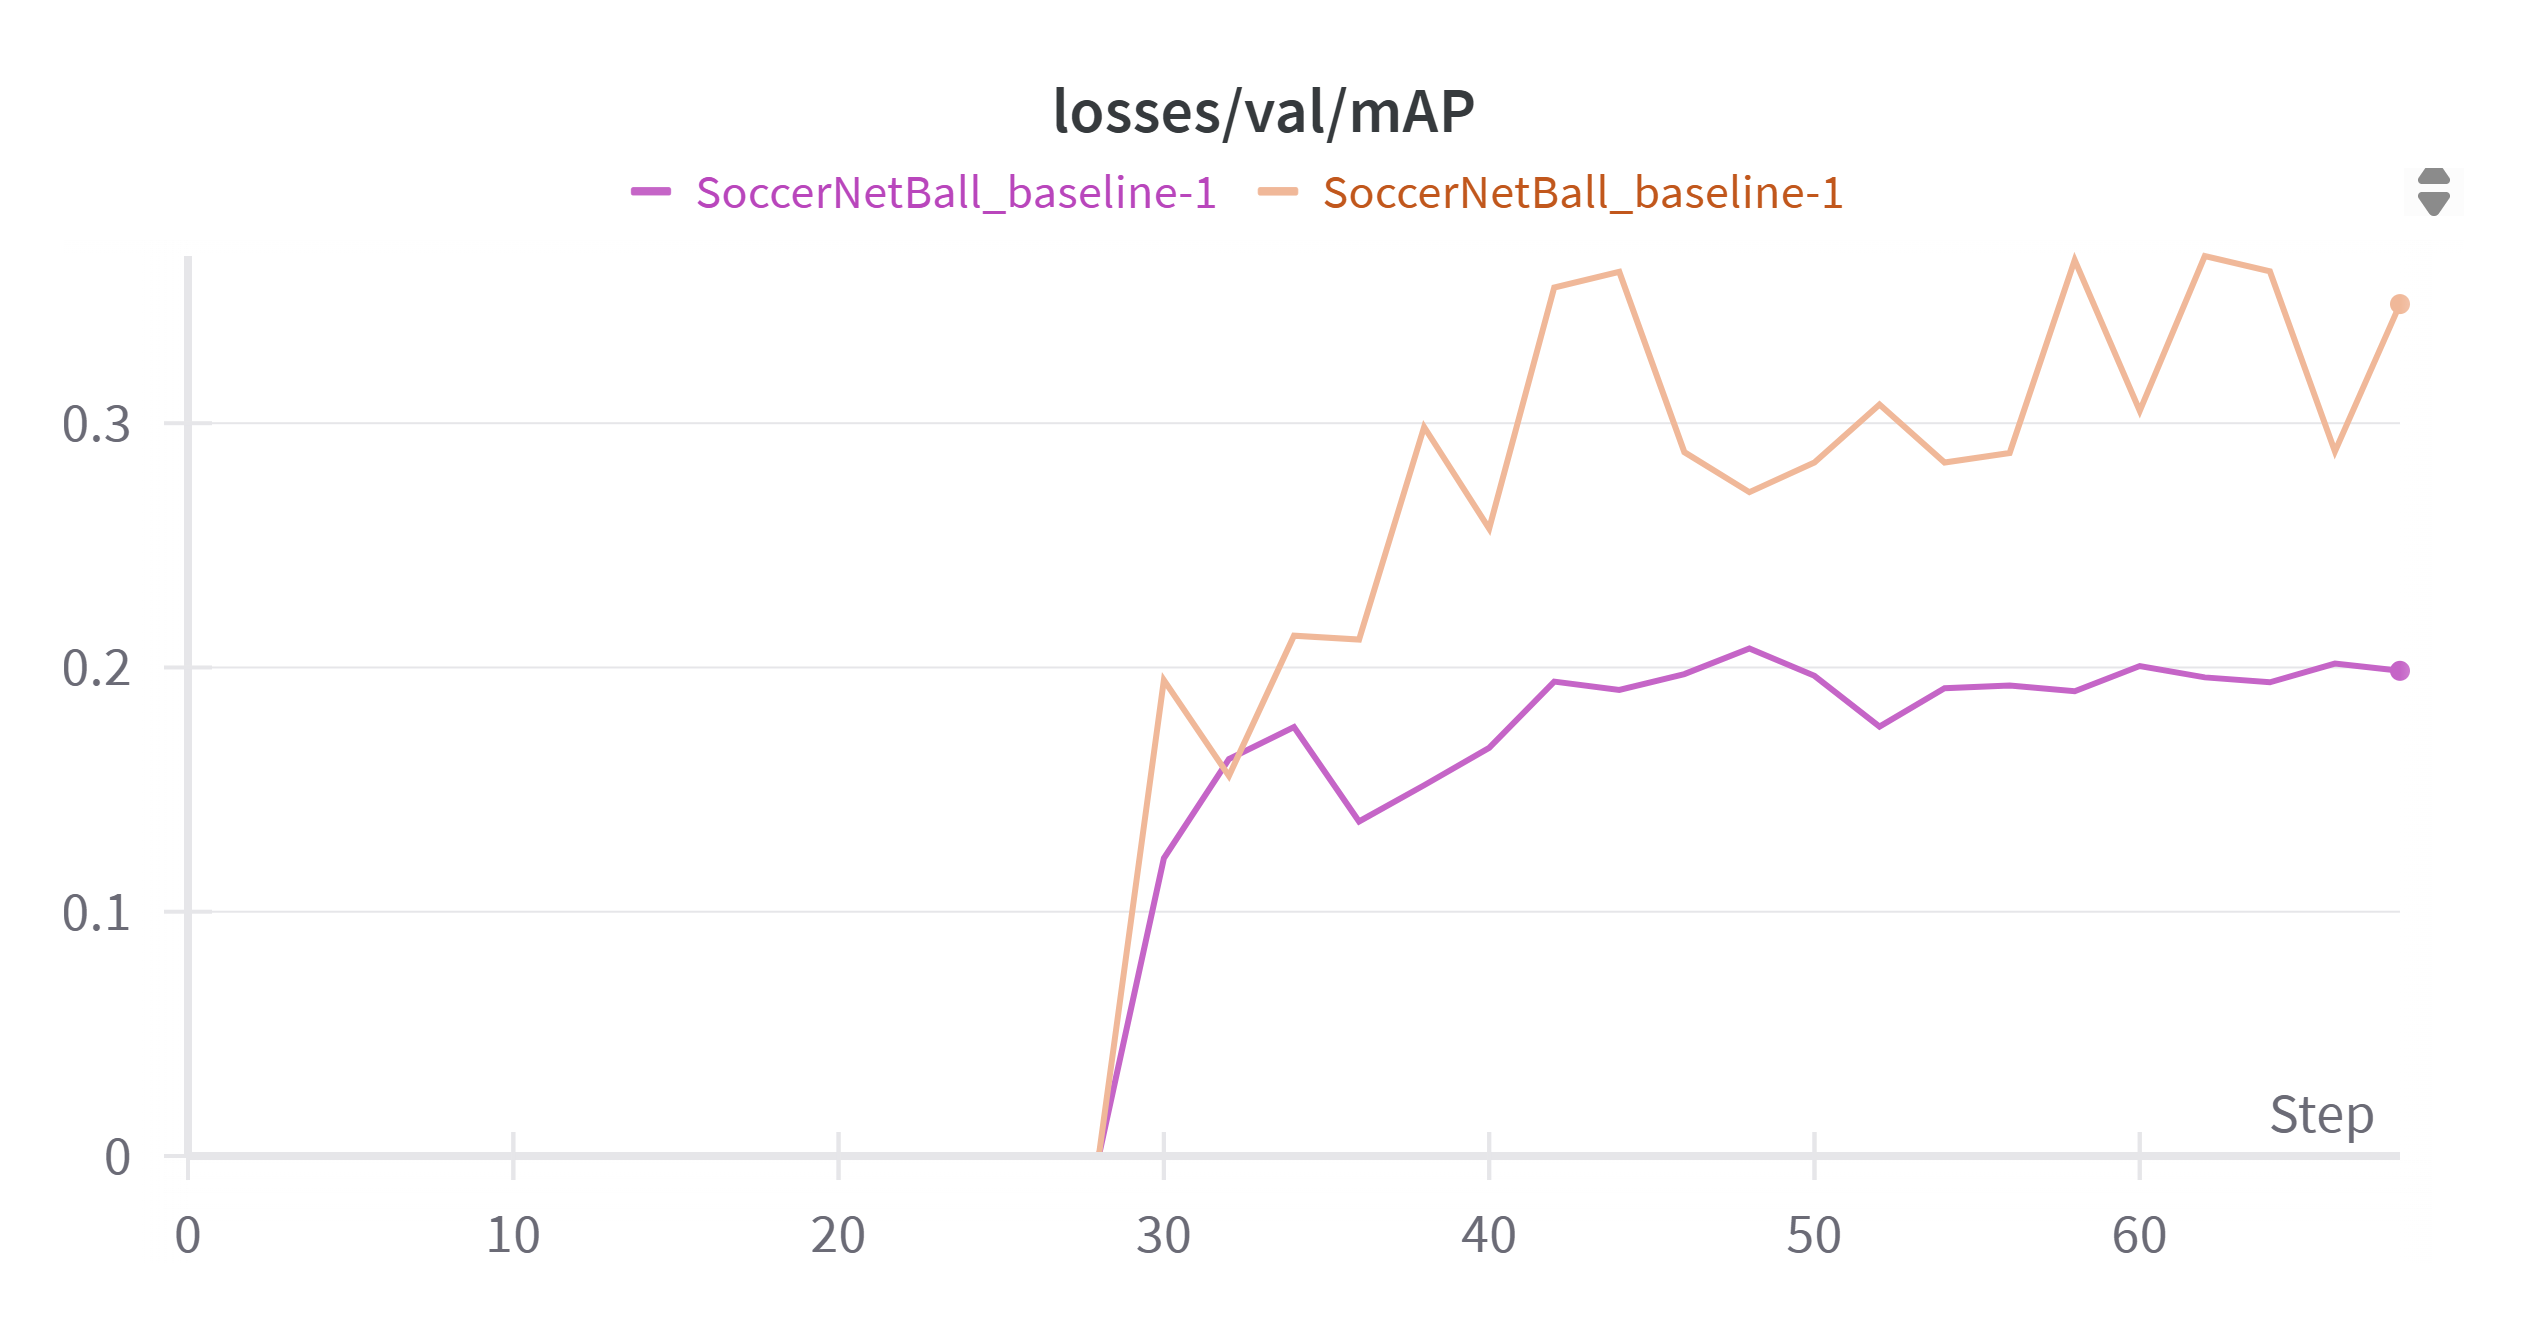
\includegraphics[width=0.75\linewidth]{figures/500_7_val_compare.png}
    \caption{Validation per epoch for the model trained with joint training (507 videos) (brown) and the model trained without joint training (purple). The models achieved a max \acrshort{map} of $36.84\%$ and $20.78\%$. }
    \label{fig:500_7_val_compare}
\end{figure}


\begin{figure}
  \begin{subfigure}{0.5\textwidth}
    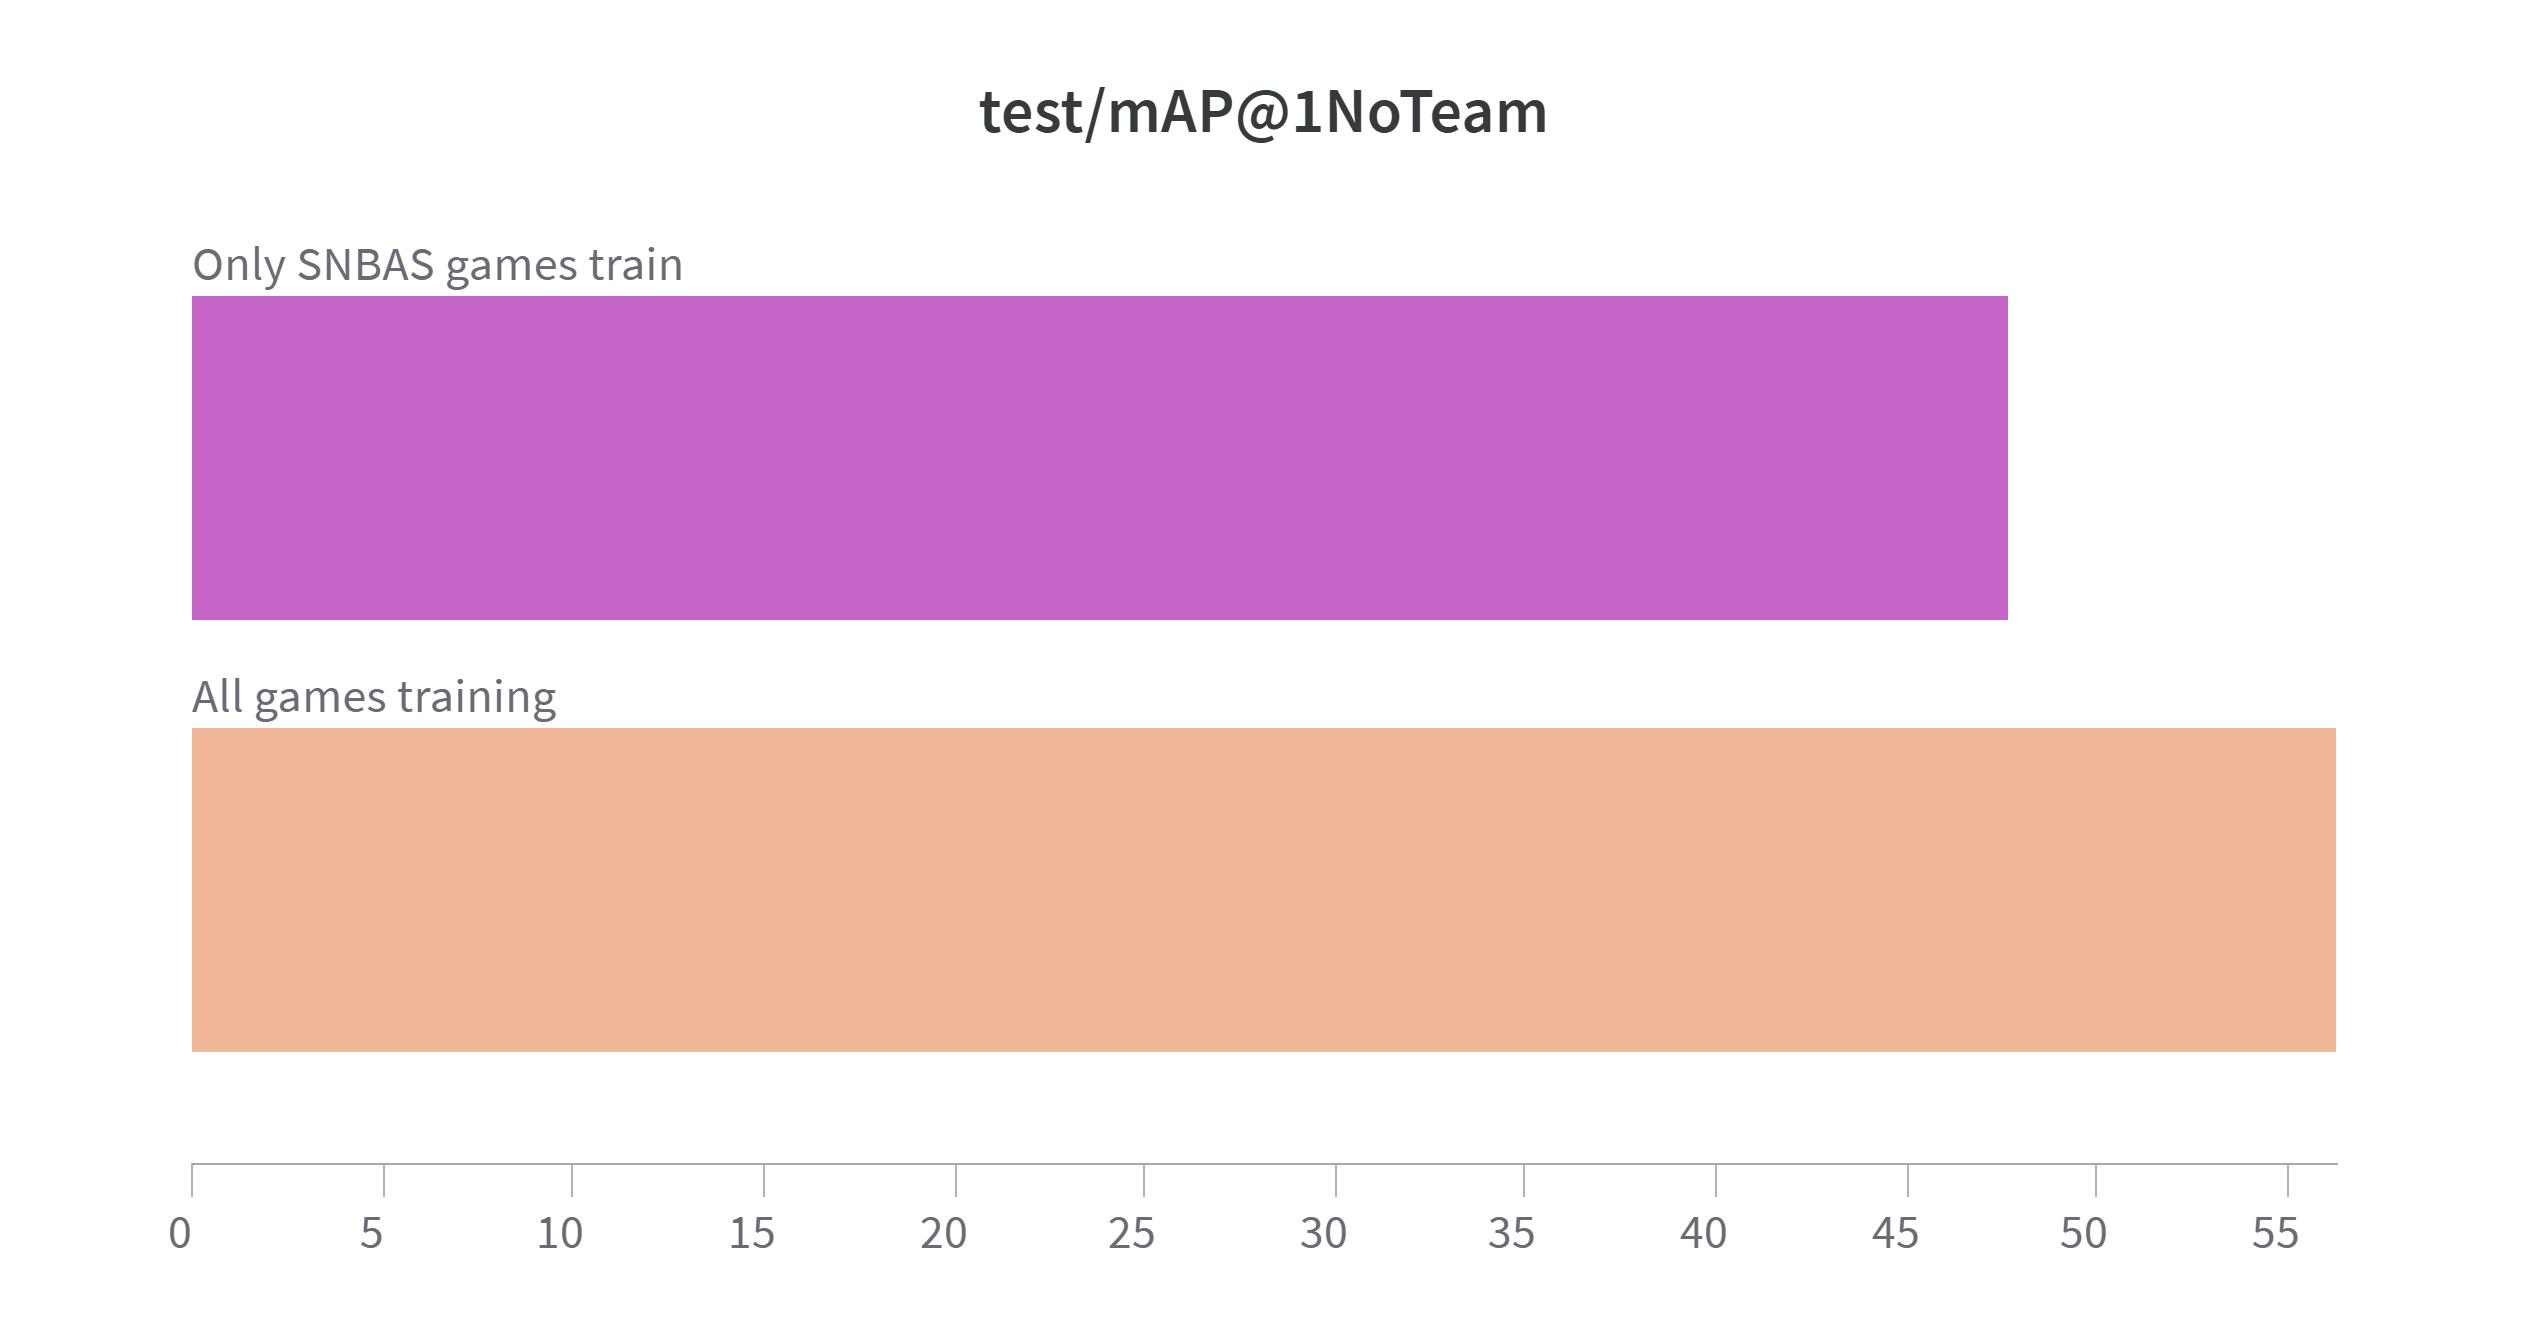
\includegraphics[width=\linewidth]{figures/total_map_no_team.png}
    \caption{The \acrshort{snb} training achieved a $47.65\%$ accuracy, the full training achieved $56.26\%$ when ignoring team prediction. }
    \label{fig:tdeed_map_no_team}
  \end{subfigure}%
  \hspace*{\fill}   % maximize separation between the subfigures
  \begin{subfigure}{0.5\textwidth}
    \centering
    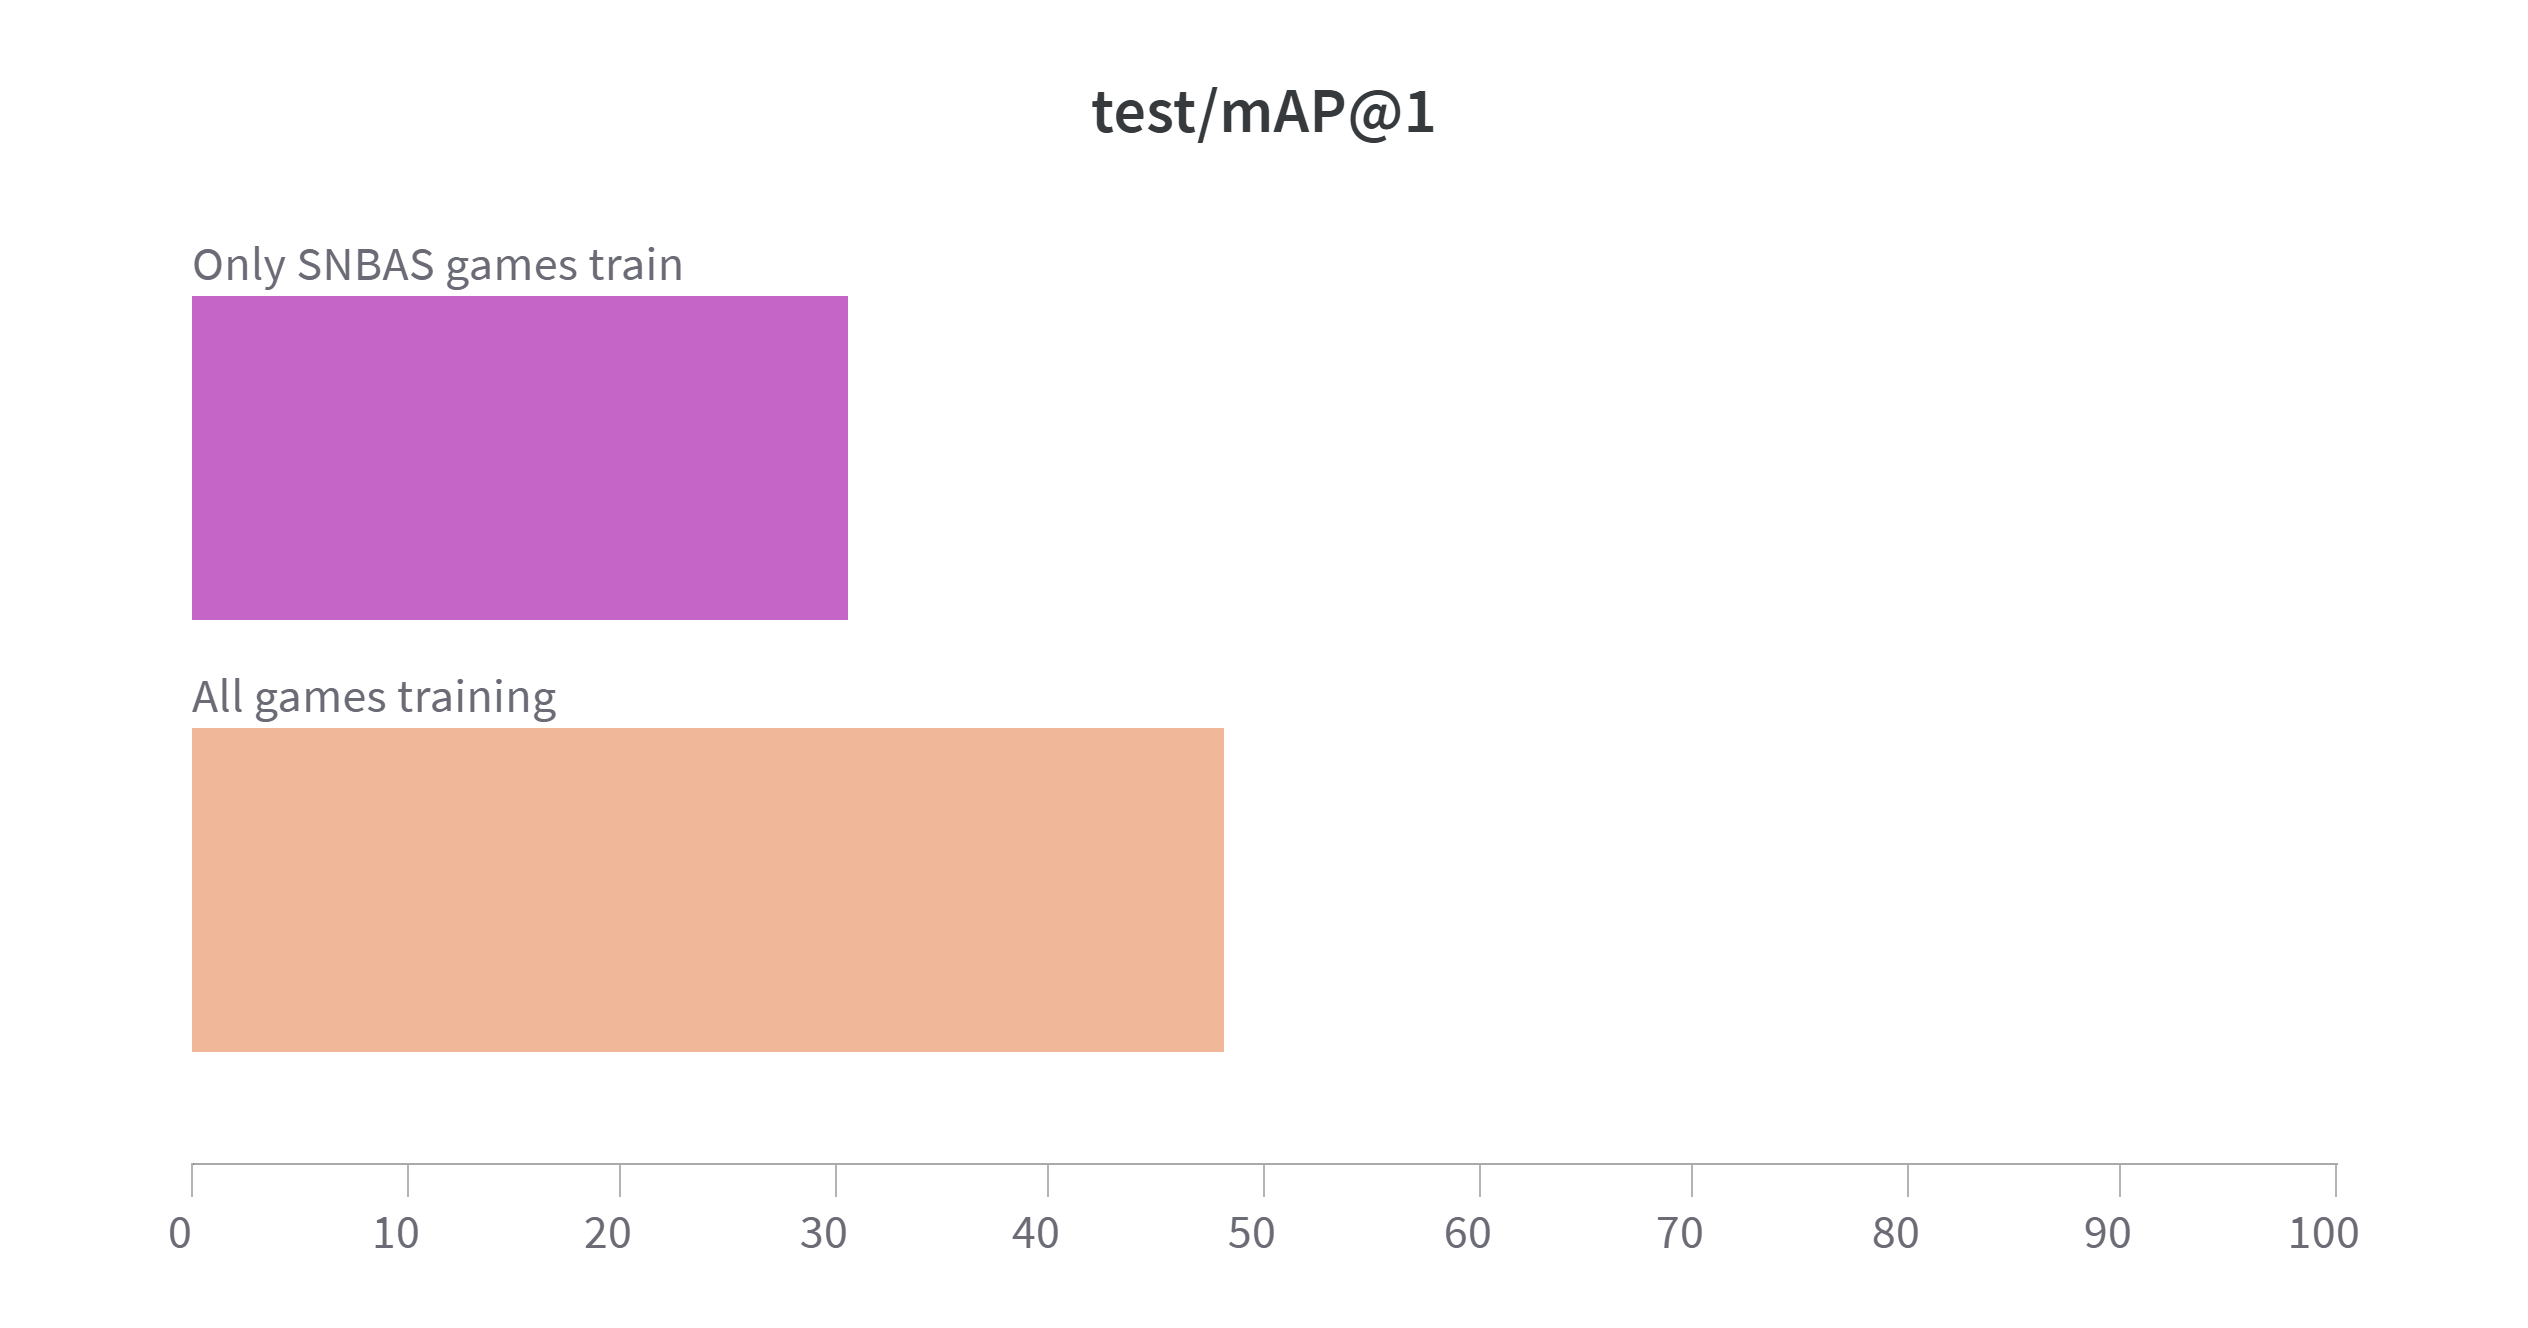
\includegraphics[width=\linewidth]{figures/total_map.png}
    \caption{The \acrshort{snb} and full model achived $30.62\%$ and $48.18\%$ respectively when  predicting teams. }
    \label{fig:map_team}
  \end{subfigure}%
  \hspace*{\fill}  
  \caption{The test-\acrshort{map} for the two models. The full training performed better in both categories, with and without team prediction. The difference was significant in both cases, but the difference increased when including the team predictions.}
  \label{fig:tdeed_map}
\end{figure}

\begin{figure}
    \centering
    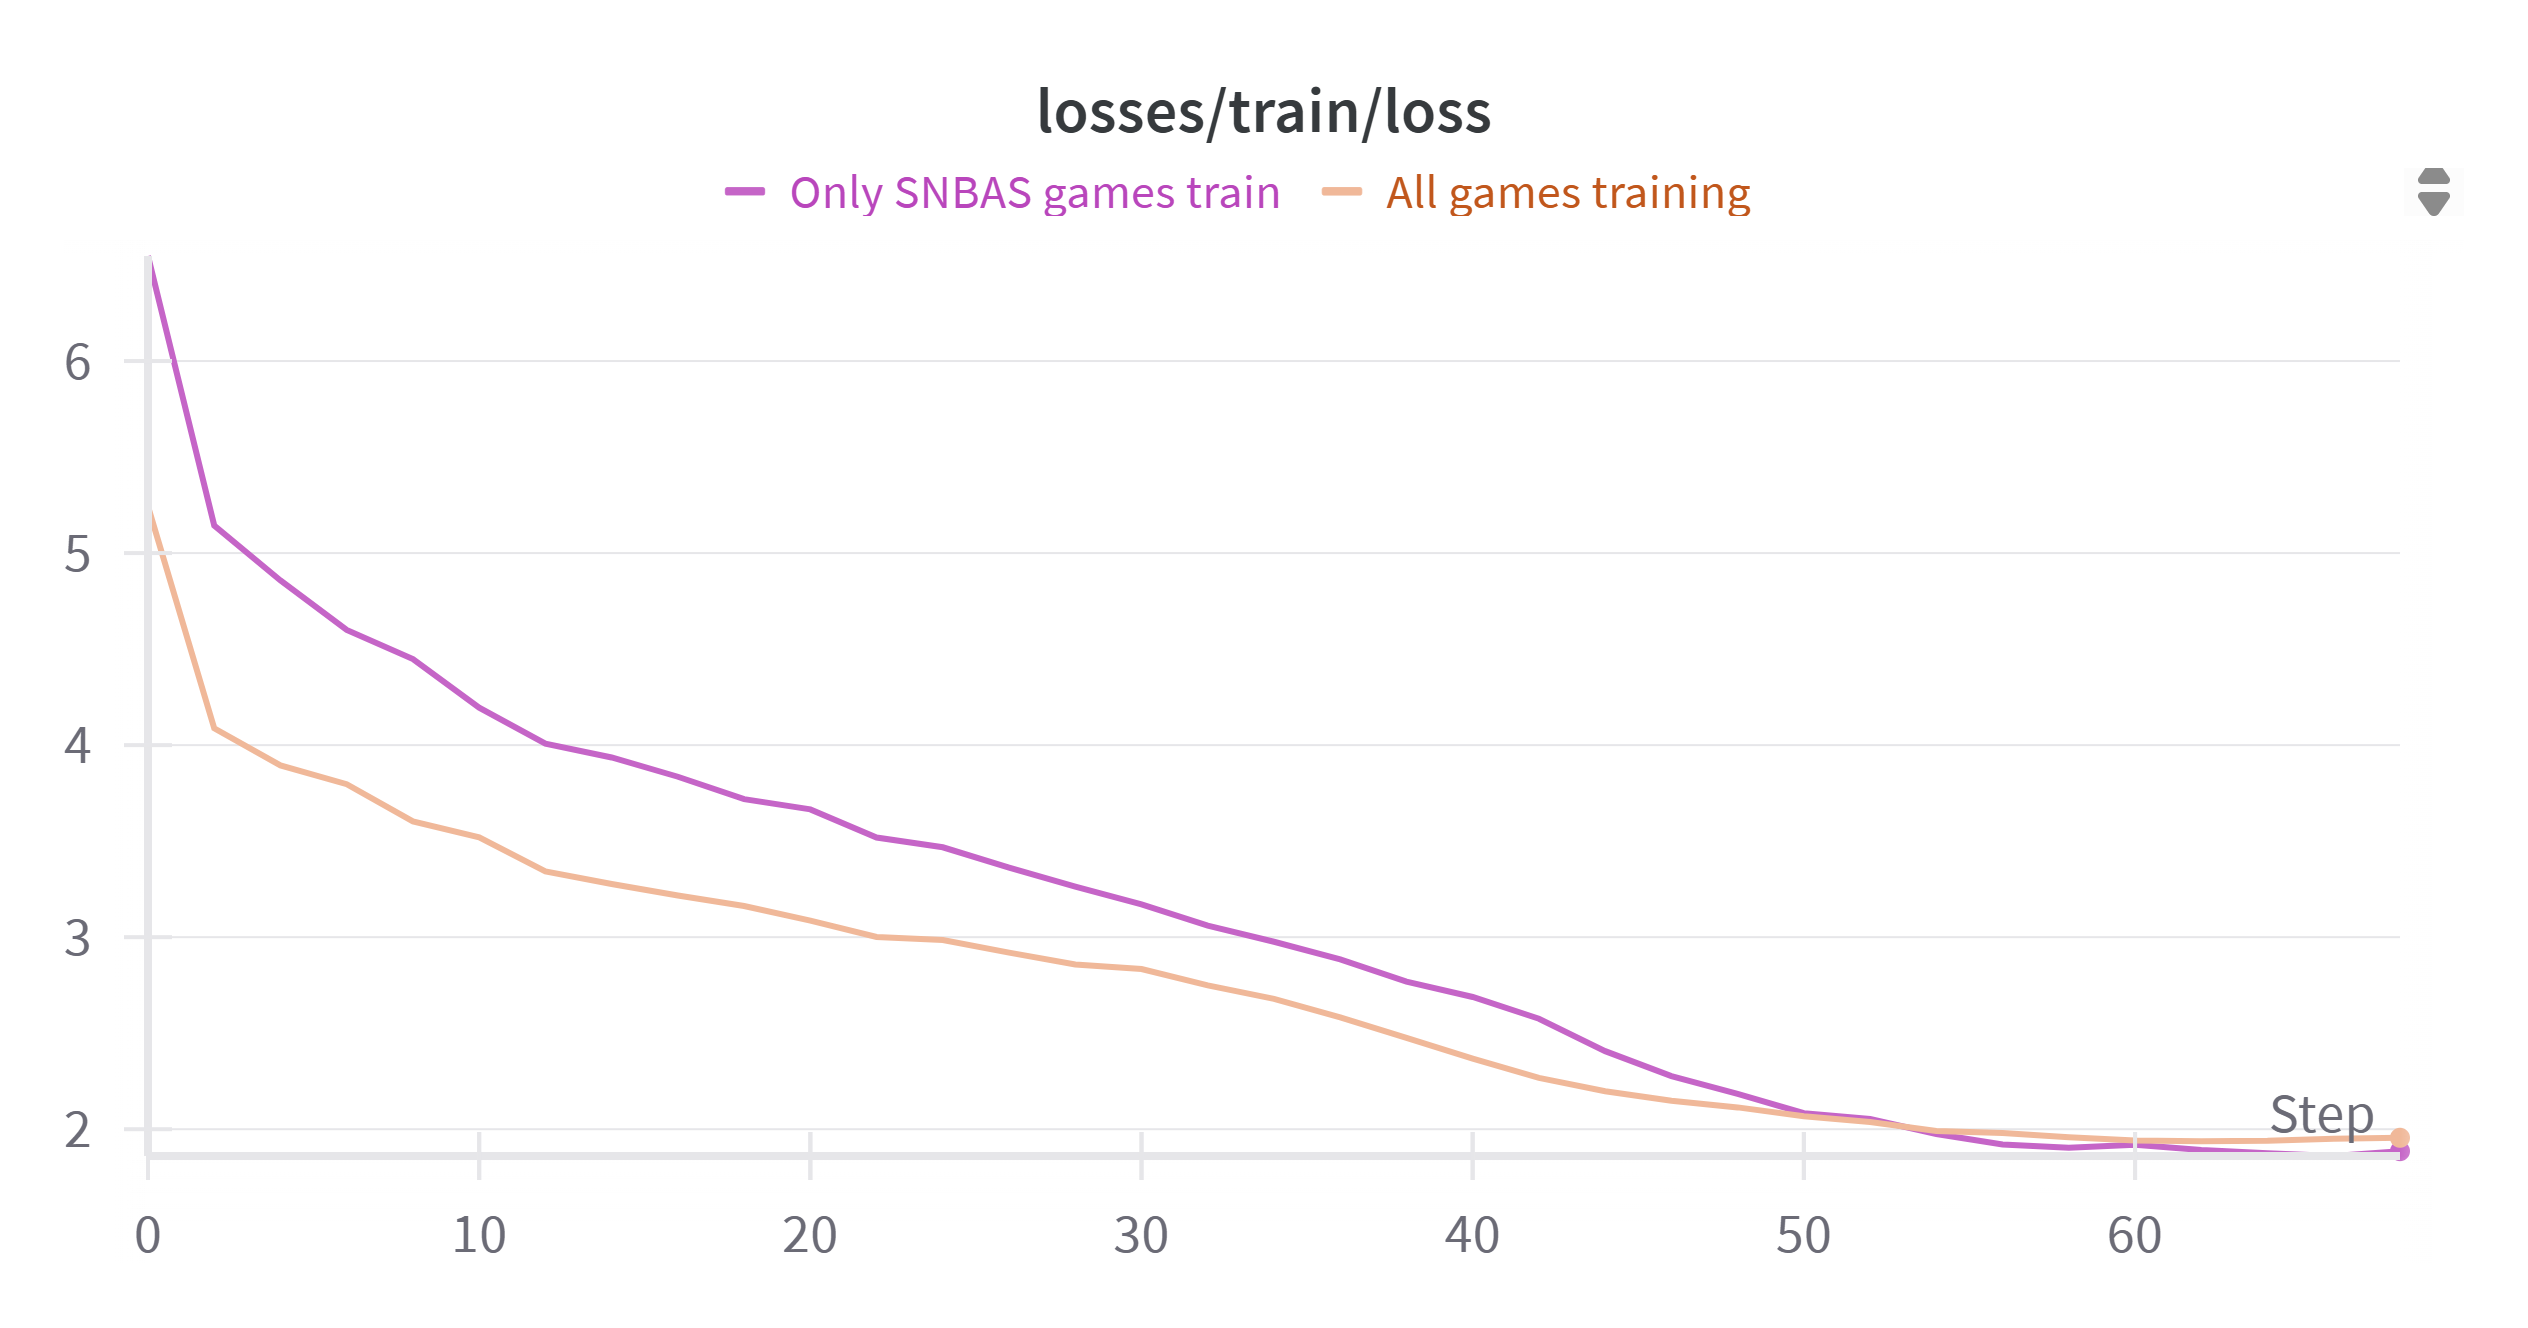
\includegraphics[width=0.5\linewidth]{figures/tdeed_train_loss.png}
    \caption{Training loss. The loss for all games is generally lower before both models converge at the same loss towards the end. }
    \label{fig:tdeed_train_loss}
\end{figure}

The results are showed in \cref{fig:500_7_val_compare,fig:tdeed_map_no_team,fig:map_team,fig:tdeed_train_loss} as direct comparisons. The results show that the model with more training data performs better in all metrics, even though it is in a different annotation format. The biggest difference comes when predicting the team, class, and time in \cref{fig:tdeed_map_no_team}.

\subsection{Discussion}
\label{ssec:ex5_discussion}

The most evident result is that the \acrshort{tdeed} model trained with more data (507 videos, "joint training") significantly outperforms the model trained only on \acrshort{snb} games. The performance gains align with general machine learning principles, which suggest that more data yields better performance. The substantial jump shown in \cref{fig:tdeed_map} shows how the model trained on more data performs significantly better in the most complex task. All reported metrics report substantially better performance for the bigger model. 

Interestingly, the difference increases when the team's prediction is added. The large old dataset does not have annotations for teams. This indicates that the model learns useful features for identifying teams based solely on game observations. This ability is extended to the realm where team matters. The difference in \acrshort{map} is doubled when adding team prediction, highlighting its importance. Without targeted experiments, it is difficult to pinpoint precisely where the difference originates.  

While the range of event types differs for the datasets, the information about events is more detailed. The belief is that the model uses game context to predict events. Football actions are highly dependent on what action occurred before and what action will occur next. 

The fact that both models eventually converge to a similar loss suggests that, given enough training, both can fit their respective training datasets similarly. However, the initial lower loss for the model with more data suggests it gets a "head start" in this fitting process, likely due to the increased volume and richness of information available from the outset. The difference in validation and test scores underlines the idea of the richer context learned from the larger dataset. The model has better generalization. 

Experiment 5 aligns with the philosophy behind pretraining and transfer learning. Large-scale data helps build better, more generalizable models. While achieving the same loss on the training data, the validation scores are significantly better for the better-trained model, which demonstrates its generalizability. Training in the football domain favors quantity and diversity, even with some annotation inconsistencies or variations in depth, over smaller, perfectly tailored datasets.

\section{Experiment 6: Testing validation stride and postprocessing of \acrshort{tdeed}}
\label{sec:experiment_6}

This experiment is motivated by earlier results that suggested postprocessing steps could lead to significant performance improvements. 

\subsection{Setup}
\label{ssec:ex6_setup}
The setup is similar to that in \cref{sec:experiment_5}, where a small, new dataset is utilized. The only difference in these runs is:

\begin{itemize}
    \item \textbf{Stride} is set to one, not two, as in the baseline.
    \item \textbf{Postprocessing} is disabled, the baseline uses \acrlong{snms}.
\end{itemize}

\subsection{Results}
\label{ssec:ex6_results}

\begin{figure}
    \centering
    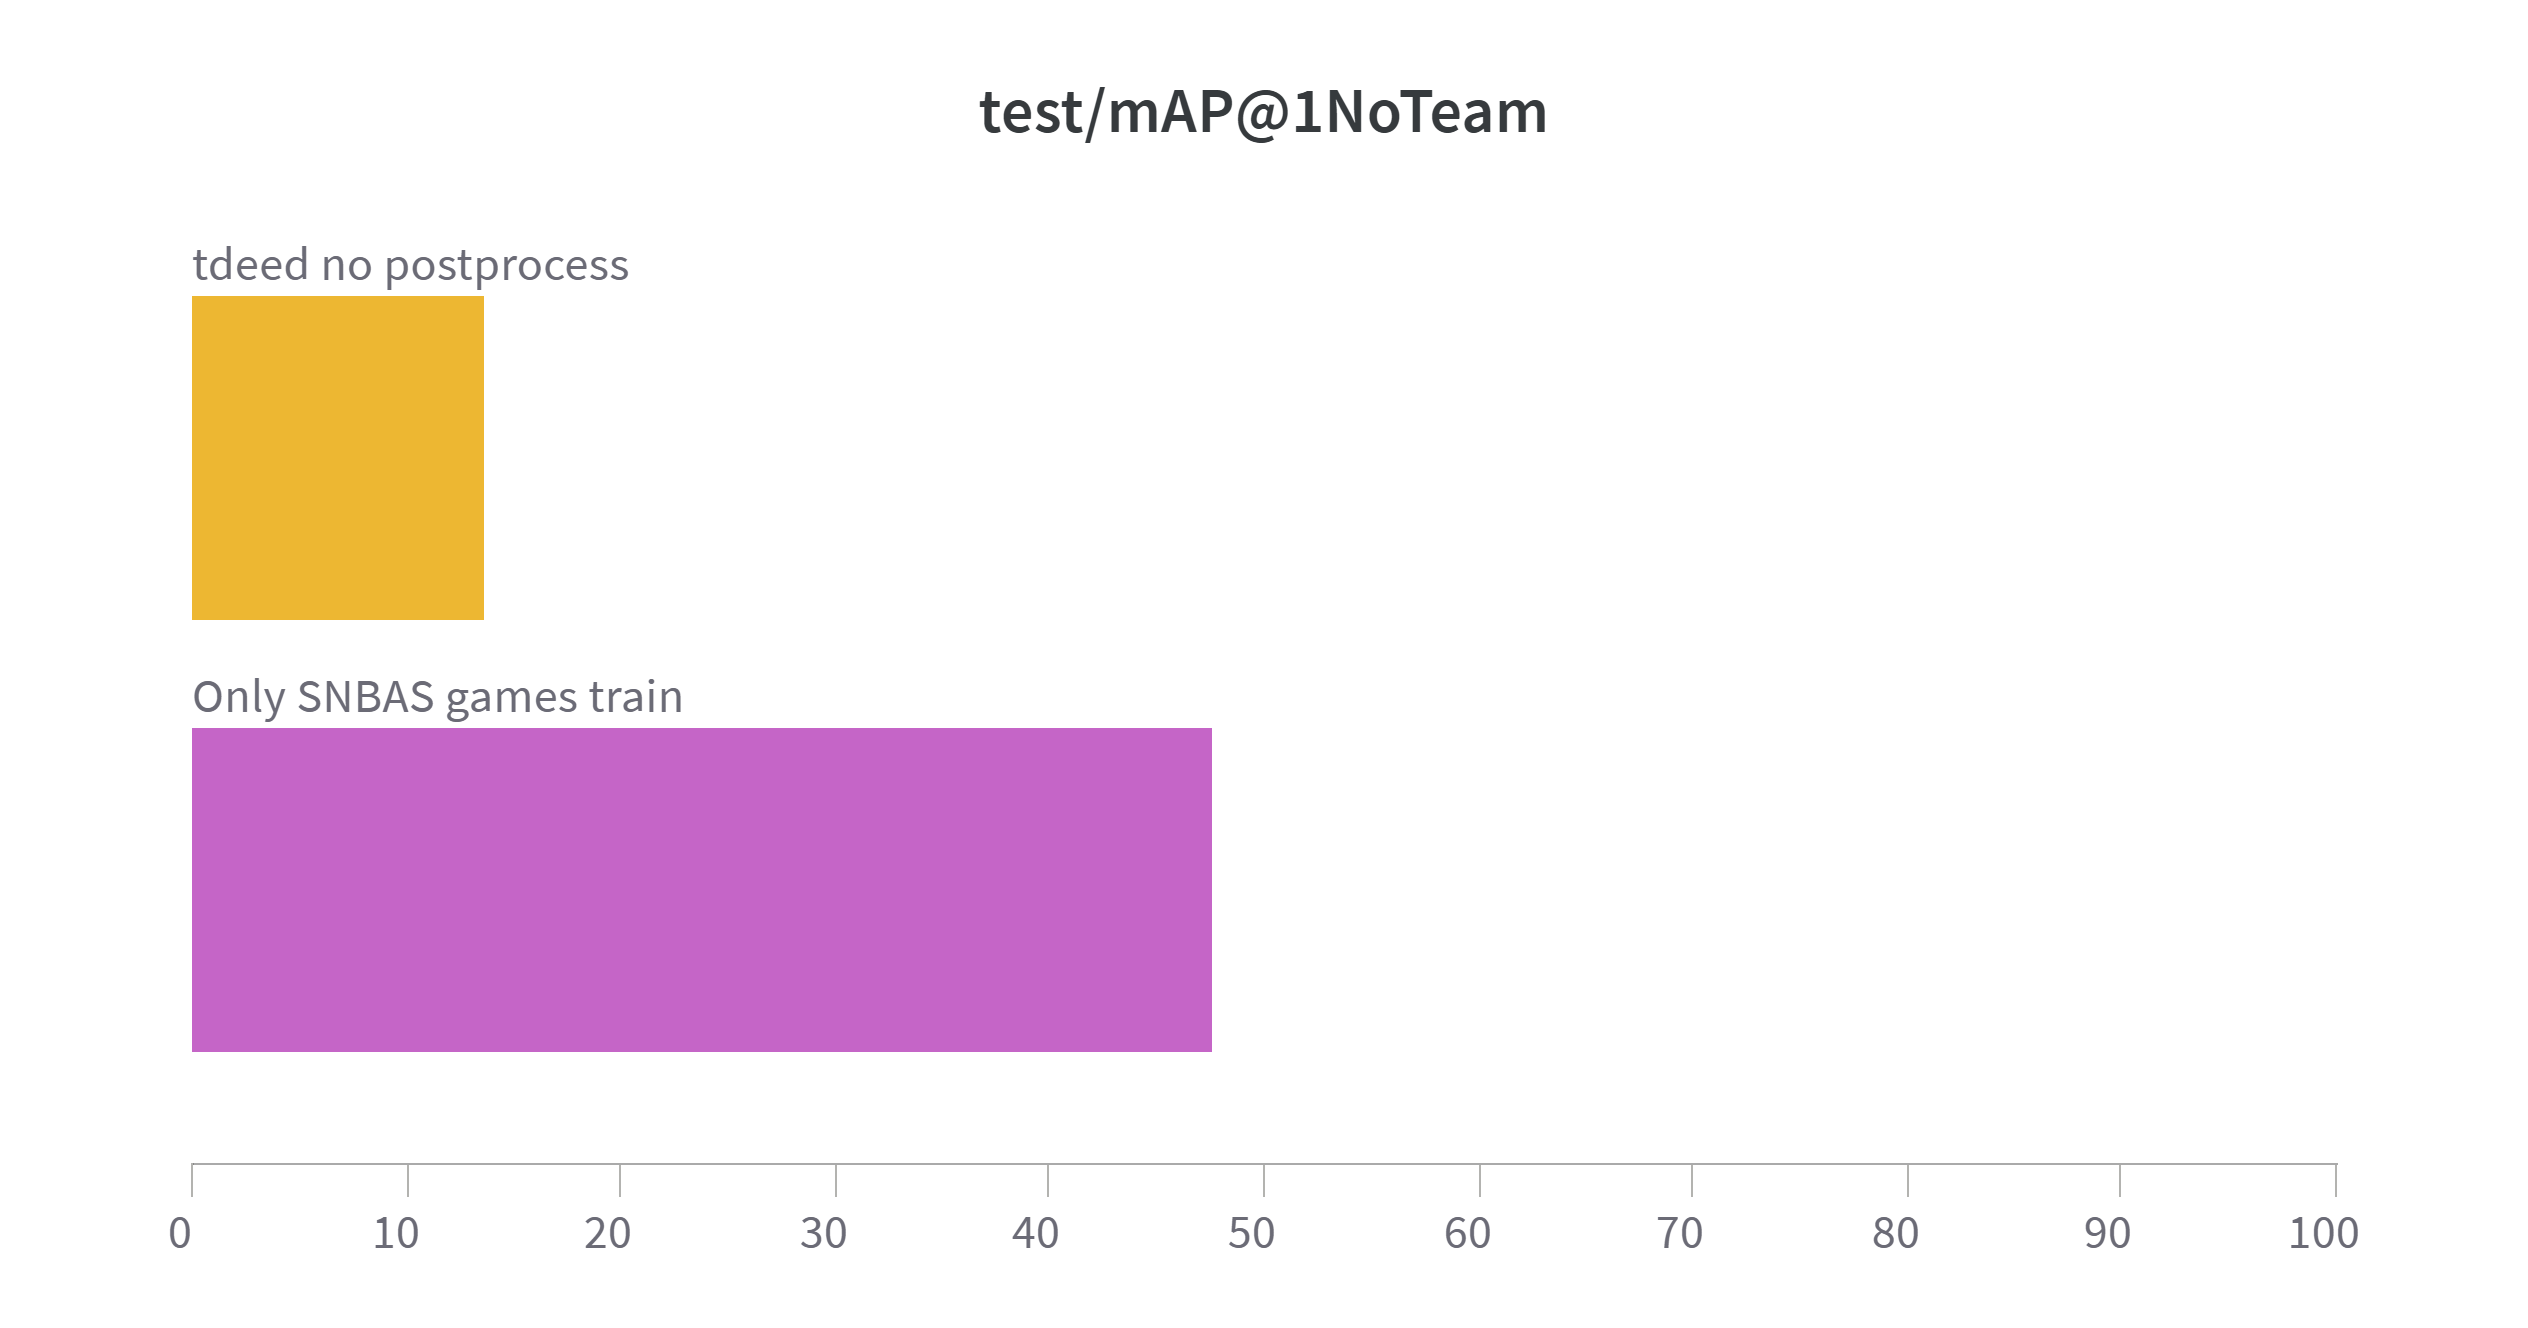
\includegraphics[width=0.75\linewidth]{figures/no_pprocess_test.png}
    \caption{Test results on the models. The figure shows the big impact of applying the postprocessing step. The test results of each model are $13.62\%$ and $47.65\%$, respectively. Both cases use $stride=1$.}
    \label{fig:ex6:no_pp_test}
\end{figure}

\begin{figure}
    \centering
    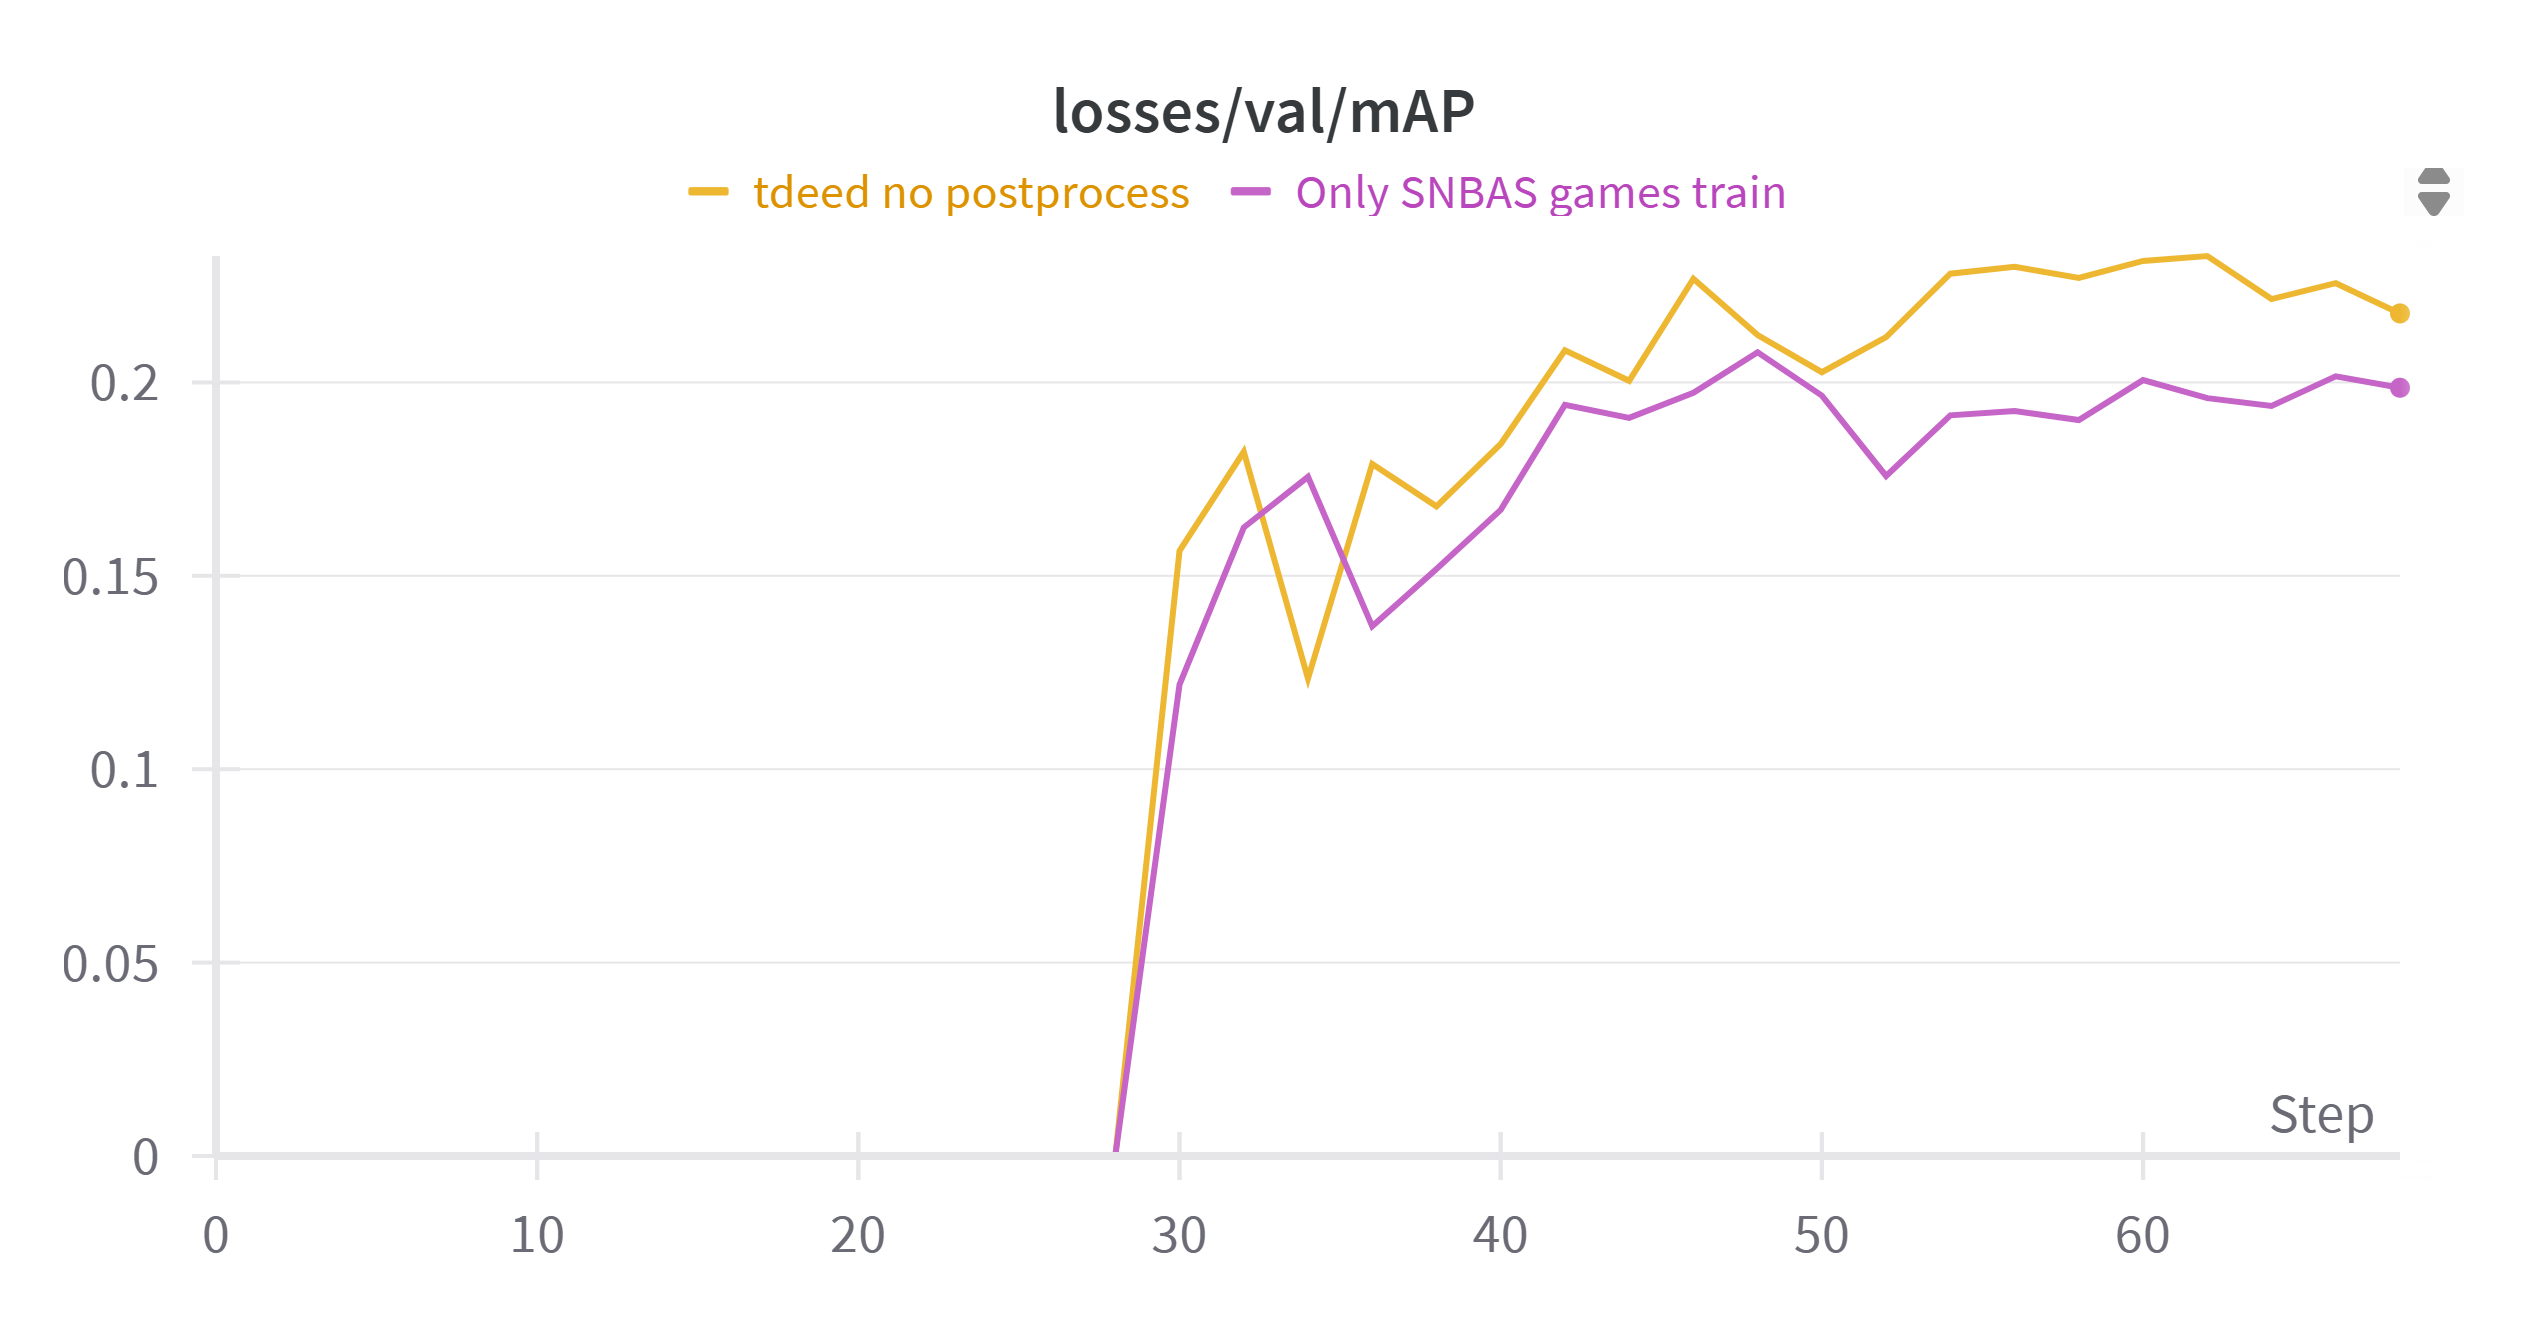
\includegraphics[width=0.75\linewidth]{figures/no_pprocess_val.png}
    \caption{The development of validation scores over the training session. After the first five validation epochs, where the results vary, the model with a lower validation stride is better. Their peaks at epoch 23 and 24, top out at $22.68\%$ and $20.78\%$. }
        \label{fig:ex6:no_pp_val}
\end{figure}

The validation differences were slight but notable. \cref{fig:ex6:no_pp_val} shows how the scores develop over time, and that their peaks vary not much in value. As seen in \cref{fig:ex6:no_pp_avg_val}, the difference in validation score increases as the training continues. 

\begin{figure}
    \centering
    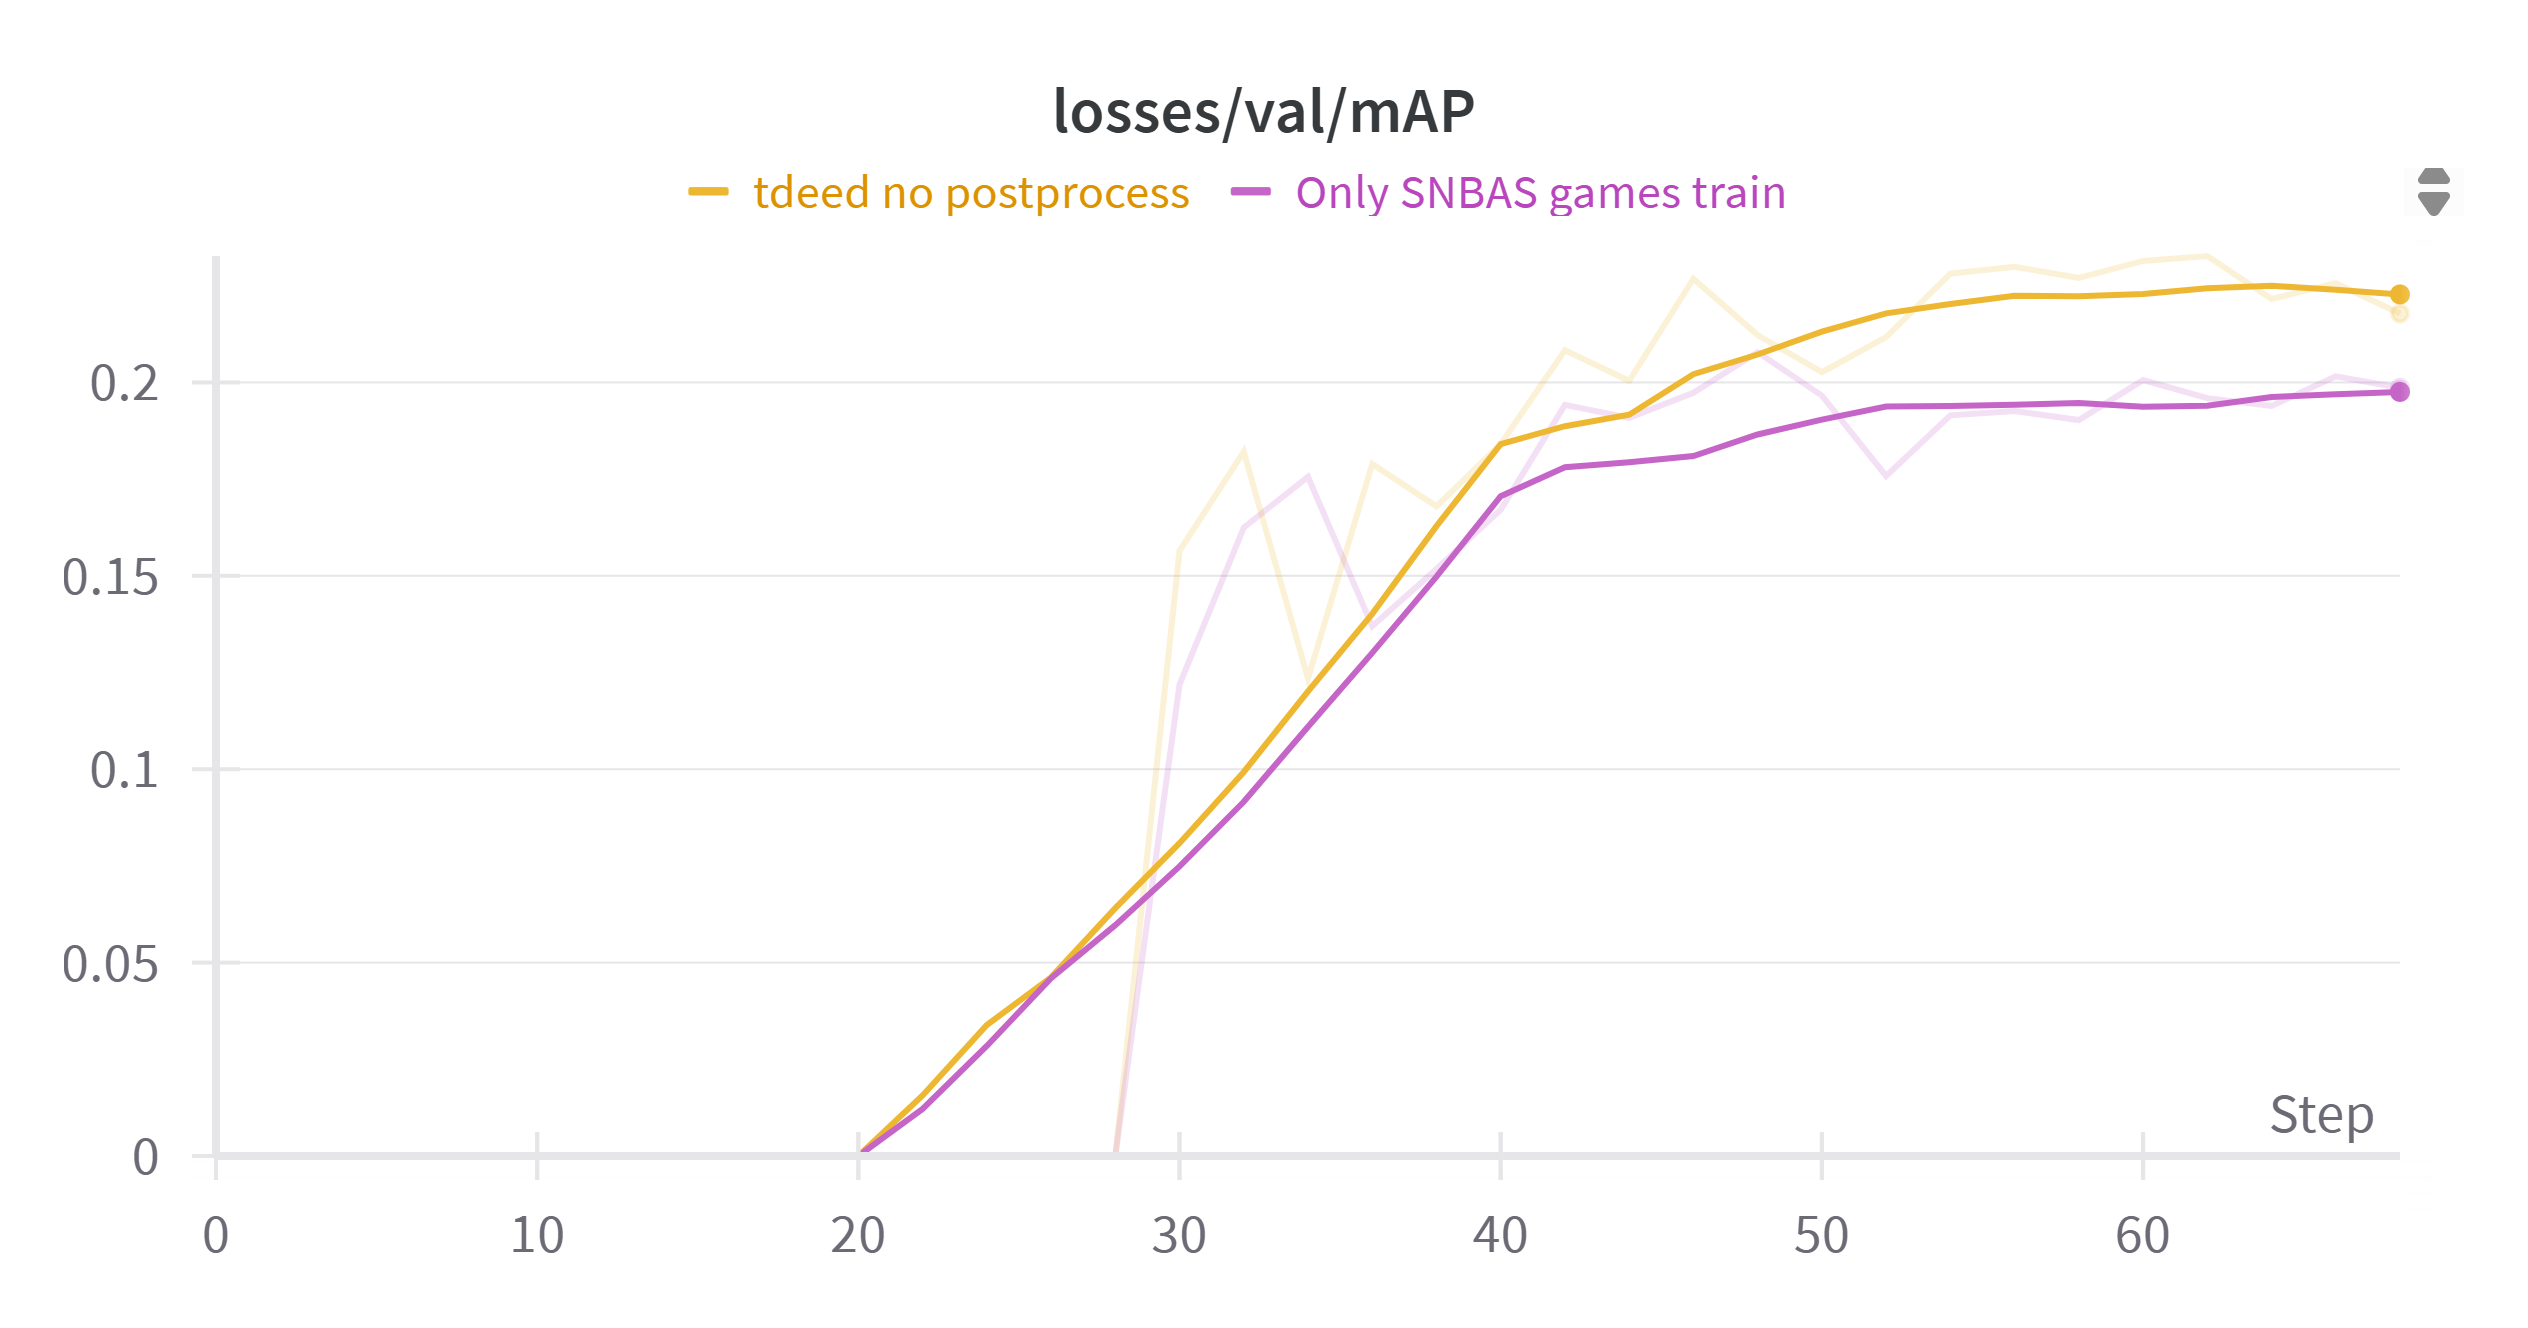
\includegraphics[width=0.75\linewidth]{figures/no_pprocess_avg_val.png}
    \caption{The same graph as in \cref{fig:ex6:no_pp_val}, but with the running average, not validation per epoch.}
    \label{fig:ex6:no_pp_avg_val}
\end{figure}

\begin{figure}
    \centering
    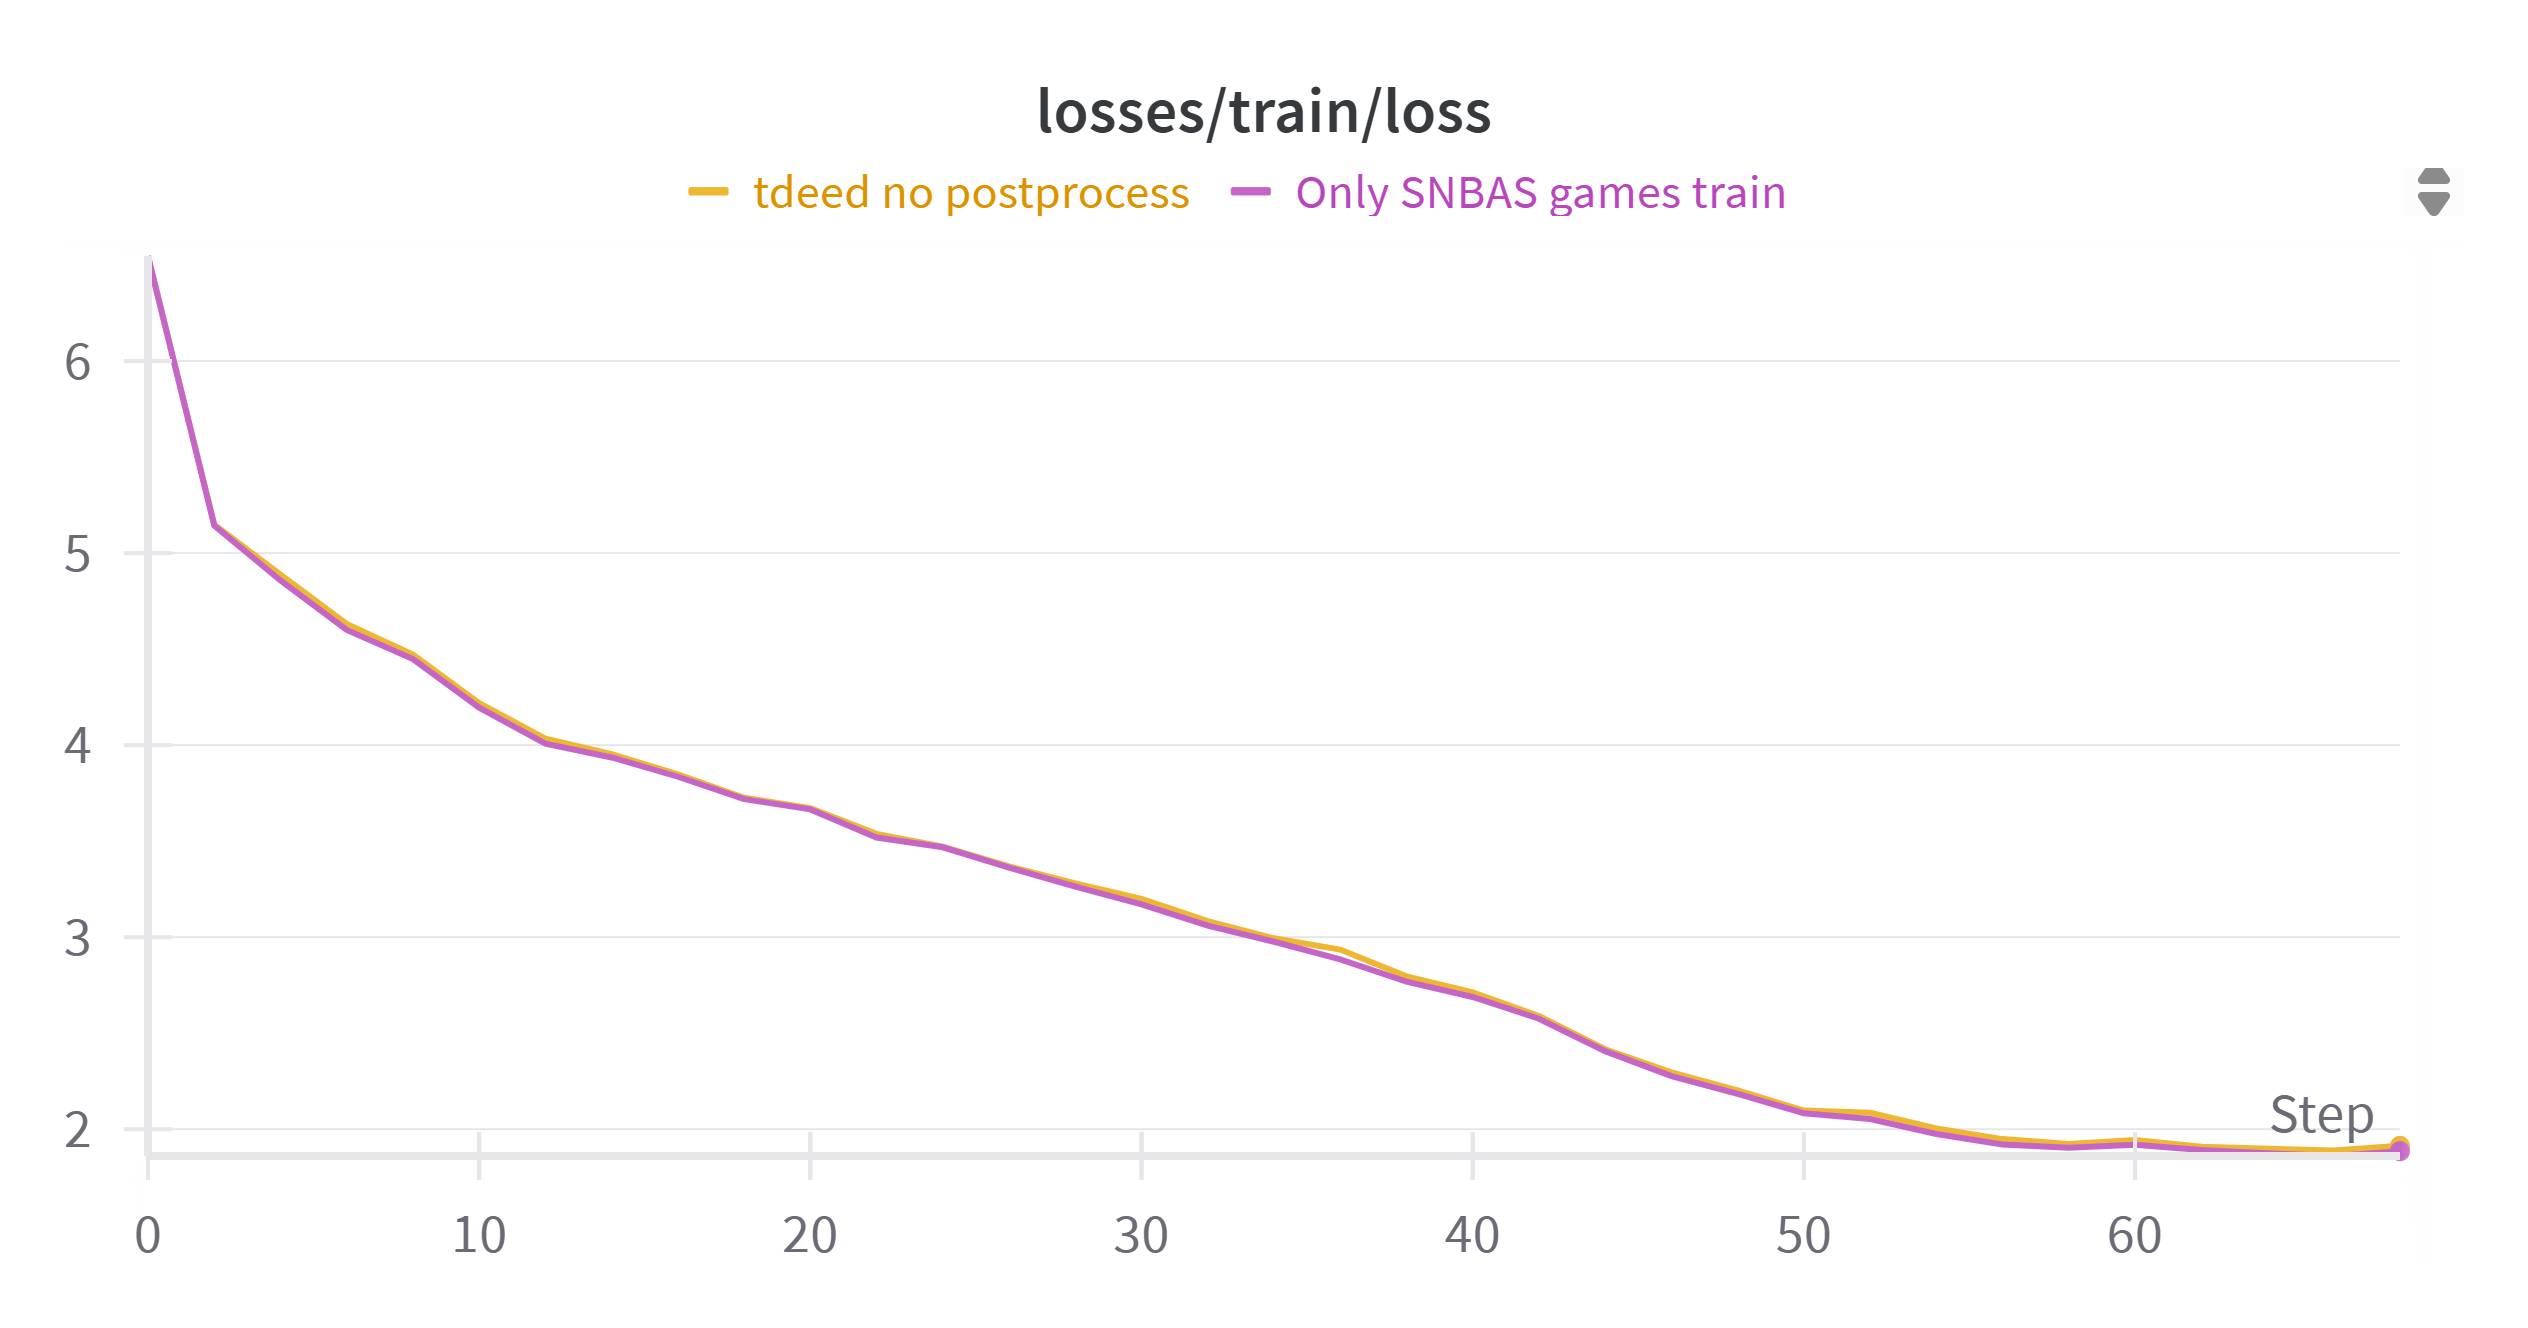
\includegraphics[width=0.75\linewidth]{figures/no_pprocess_loss.png}
    \caption{Loss scores for the two trainings. As expected, it is equal because only validation and test scores should vary.}
    \label{fig:ex6:no_pp_loss}
\end{figure}

The difference in test scores, \cref{fig:ex6:no_pp_test}, is significant. The model with postprocessing performs more than three times better than the model without postprocessing. If one recalls \cref{fig:tdeed_map_no_team}, the difference to the training model on the full dataset is $42.64\%$. 

\subsection{Discussion}
\label{ssec:ex6_discussion}

\acrfull{snms} is critical for \acrshort{tdeed}'s performance because the raw output likely contains many redundant and overlapping detections for the same event. The drop off when removing \acrshort{snms} is massive. Experiment 6 provides evidence that the validation score in Experiment 1 was significantly tampered with by the lack of \acrshort{snms}. The validation scores can not be directly compared from raw \acrshort{tdeed} to \acrshort{vms}. 

I did not expect the significance of the postprocessing to be as considerable as it was, and subsequently, the impact of the validation step to be so little. The importance could be greater if the model did not provide as many redundant, overlapping predictions. There is an increase from $stride=2$ to $stride=1$ of $3\%$. A theory is that with such an acceptable margin of $\pm1s$, and the sheer number of predictions, more predictions fit within the constraints. There should be no difference in the number of actions predicted, but rather in the temporal accuracy. 

This experiment confirms that \acrshort{snms} is the primary driver behind the increase from the validation to the test score. The stride change had a small but noticeable difference in validation. However, the change was insignificant compared to the improvement from the postprocessing. After changing stride, the results were not comparable with \acrshort{vms}. 

The high impact from \acrshort{snms} could be because of the benchmark specificity. Because each event can only be assigned to one ground truth, many predictions around one ground truth will cause a low \acrlong{map}. For a detection system with $k$ redundant predictions per true object, the precision becomes:

\[P_{redundant} = \frac{TP}{TP + (k-1) \cdot TP} = \frac{1}{k}\]

This necessitates non-maximum suppression for a good result, as increasing $k$ reduces precision. 

% With validation results yielding different results, integrating postprocessing into the validation step must be discussed. Even if time-consuming, this step is necessary to conduct a thorough hyperparameter search and obtain reliable estimates of test results. 

Early stopping mechanisms based on validation scores might perform suboptimally because of the lack of postprocessing. 

The findings and the clarification about the redundant positive predictions decrease the \acrshort{map} score of validation.

\section{Summary}

Experiment one compared \acrfull{vms} and \acrfull{tdeed}, finding it difficult to compare the two due to postprocessing. However, the model is likely more accurate with \acrshort{tdeed} achieving a higher test score than the validation score for \acrshort{vms}. No conclusion was reached on that. Experiment two confirmed \acrshort{vms}'s significant time complexity advantages, although a slow preprocessing timeline currently hinders its practical application. Pretraining proved helpful and should be applied to the \acrshort{vms} model. Using larger context vectors increased performance similarly. Future studies should focus on postprocessing techniques rather than hyperparameters. 